% !TEX encoding = UTF-8 Unicode
\chapter{Simulation results}  \label{chap-simulation}

This chapter describes numerical simulations carried out to demonstrate and evaluate the disturbance models and observer designs described in Chapter \ref{chap-methods}. Section \ref{section:sim-RODDs} describes simulated examples of different \gls{RODD}s. Section \ref{section:sim-obs-lin} describes experiments to evaluate the two observers in estimating the states of two simulated systems, a single-input single-output (SISO) linear system with one \gls{RODD} step disturbance, followed by a 2-input, 2-output linear system with two \gls{RODD} step disturbances. Section \ref{section:sim-ore-SISO} describes an experiment to evaluate the observers on the simulated grinding circuit model with one output variable and a step disturbance in the ore feed mix. Section \ref{section:sim-ore-mimo-ctrl} describes an experiment to evaluate the observers in a multi-variable feedback control scenario with the simulated grinding circuit model.


\section{Generating RODD disturbances} \label{section:sim-RODDs}

\gls{RODD}s are easy to generate by numerical simulation.  Plot (a) in Figure \ref{fig:rodd-sim-plots} shows a random shock sequence (\ref{eq:wpk1}) of length 1000 samples generated using a pseudo-random number generator. Plots (b), (c), and (d) show step, ramp and exponential change disturbances generated with this random shock sequence using the \gls{RODD} models in (\ref{eq:RODD-step}), (\ref{eq:RODD-ramp}), and (\ref{eq:RODD-exp}). 
\begin{figure}[htp]
	\centering
	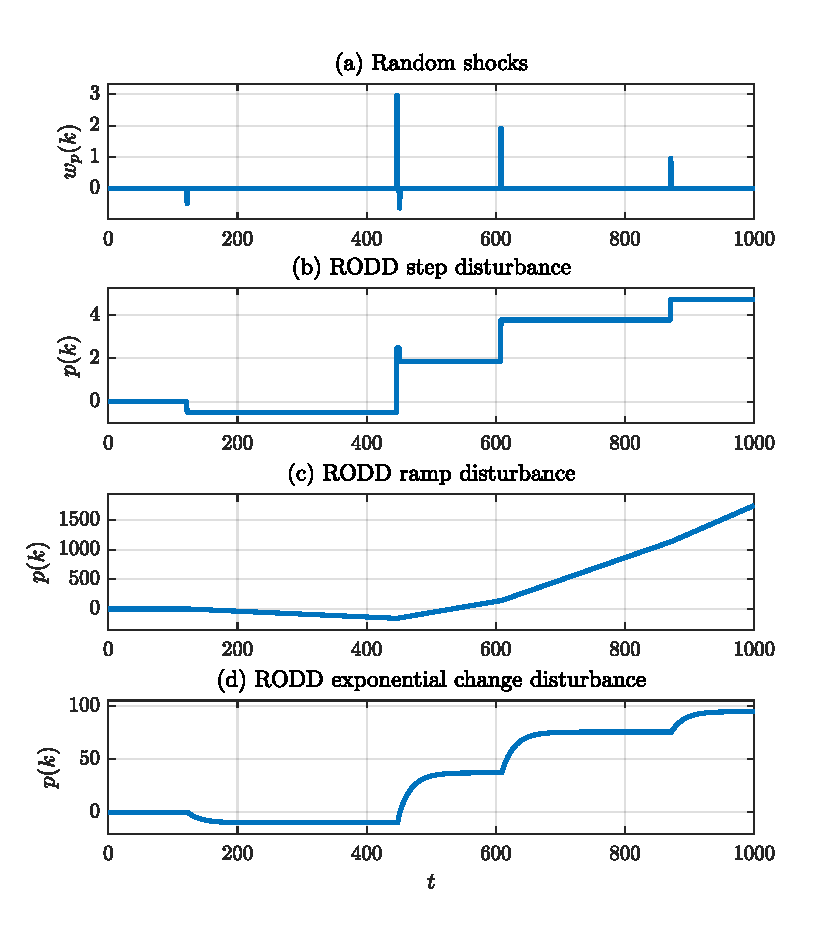
\includegraphics[width=13cm]{images/rodd_sim_plots.pdf}
	\caption{Examples of \gls{RODD}s}
	\label{fig:rodd-sim-plots}
\end{figure}
\begin{figure}[htp]
	\centering
	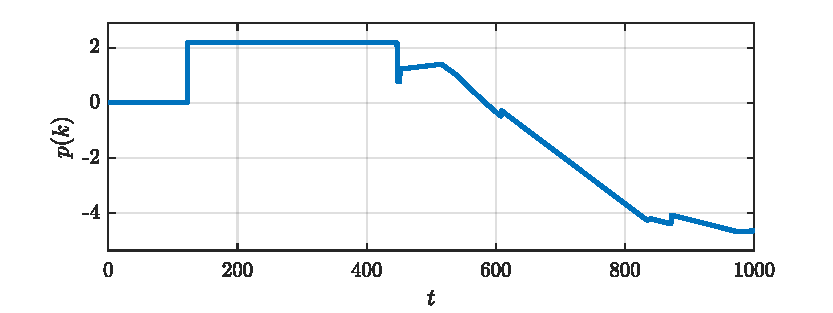
\includegraphics[width=13cm]{images/rodd_sim_plot2.pdf}
	\caption{A \gls{RODD} with steps and ramps}
	\label{fig:rodd-sim-plot2}
\end{figure}


\section{Observer evaluation with linear systems} \label{section:sim-obs-lin}

\subsection{SISO linear system} \label{sim-obs-lin-1}

To demonstrate state estimation in the presence of \gls{RODD}s, a single \gls{RODD} was simulated at the input to a SISO process represented by a discrete-time linear model, as shown in the functional diagram in Figure \ref{fig:sim-sys-diag-siso}. In addition to the unmeasured \gls{RODD}, $p(k)$, the process has a known input, $u(k)$, and a measured output, $y_M(k)$. The measurements are simulated by adding a random noise $v(k)$ with zero mean and standard deviation \glsadd{sigmaM}\gls{sigmaM} to the output of the process. At each sample time, the input and measured output are passed to an observer which calculates estimates of the process states, $\hat{\mathbf{x}}(k|k)$, and an estimate of the true process output, $\hat{y}(k|k)$.
\begin{figure}[htp]
	\centering
	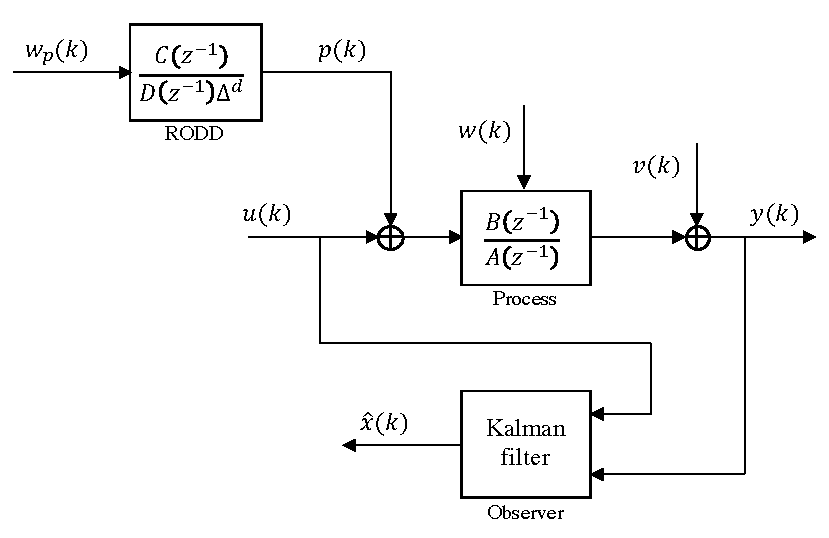
\includegraphics[width=11.5cm]{images/sim-sys-diag-siso.pdf}
	\caption{Functional diagram of the simulated SISO system with observer}
	\label{fig:sim-sys-diag-siso}
\end{figure}

For the purposes of this experiment, the linear model used to represent the process was the stable first order system,
\begin{equation}
	\frac{B(z^{-1})}{A(z^{-1})} = \frac{0.3z^{-1}}{1-0.7z^{-1}}
\end{equation}
with a sampling period of $T=0.5$.

The \gls{RODD} was a step disturbance created by setting
\begin{equation}
	\frac{C(z^{-1})}{D(z^{-1})} = \frac{1}{1-z^{-1}}.
\end{equation}
The random shock, $w_p(k)$, was defined by (\ref{eq:wpik2}) with $\epsilon=0.01$, $\sigma_{w_p}=0.01$, and $b=100$.

The state-space model used to simulate the augmented system was
\begin{equation} \label{eq:sim-sys-siso-ss-aug}
	\begin{split}
	\mathbf{x}_{a}(k+1) & =\left[\begin{array}{cc}
		0.7 & 1 \\
		0 & 1
	\end{array}\right] \mathbf{x}_{a}(k)+\left[\begin{array}{l}
		1 \\
		0
	\end{array}\right] u(k) + \mathbf{w}_{a}(k) \\
	y(k) & =\left[\begin{array}{cc}
	0.3 & 0
\end{array}\right] \mathbf{x}_{a}(k) + v(k)
\end{split}
\end{equation}
where
\begin{equation} \label{eq:sim-sys-siso-ss-aug2}
		\mathbf{x}_{a}(k) = \left[\begin{array}{l}
			x_{a,1}(k) \\
			x_{a,2}(k)
		\end{array}\right] = \left[\begin{array}{l}
		x_{1}(k) \\
		p(k)
	\end{array}\right], \mathbf{w}_{a}(k) = \left[\begin{array}{l}
	w_1(k) \\
	w_{p}(k)
\end{array}\right] .
\end{equation}

Note that with this representation, the second model state $x_{a,2}(k)$ corresponds exactly to the input disturbance $p(k)$.

\subsection{Analysis of sub-optimal estimators} \label{sim-obs-lin-1-SKF-analysis}

\begin{figure}[htp]
	\centering
	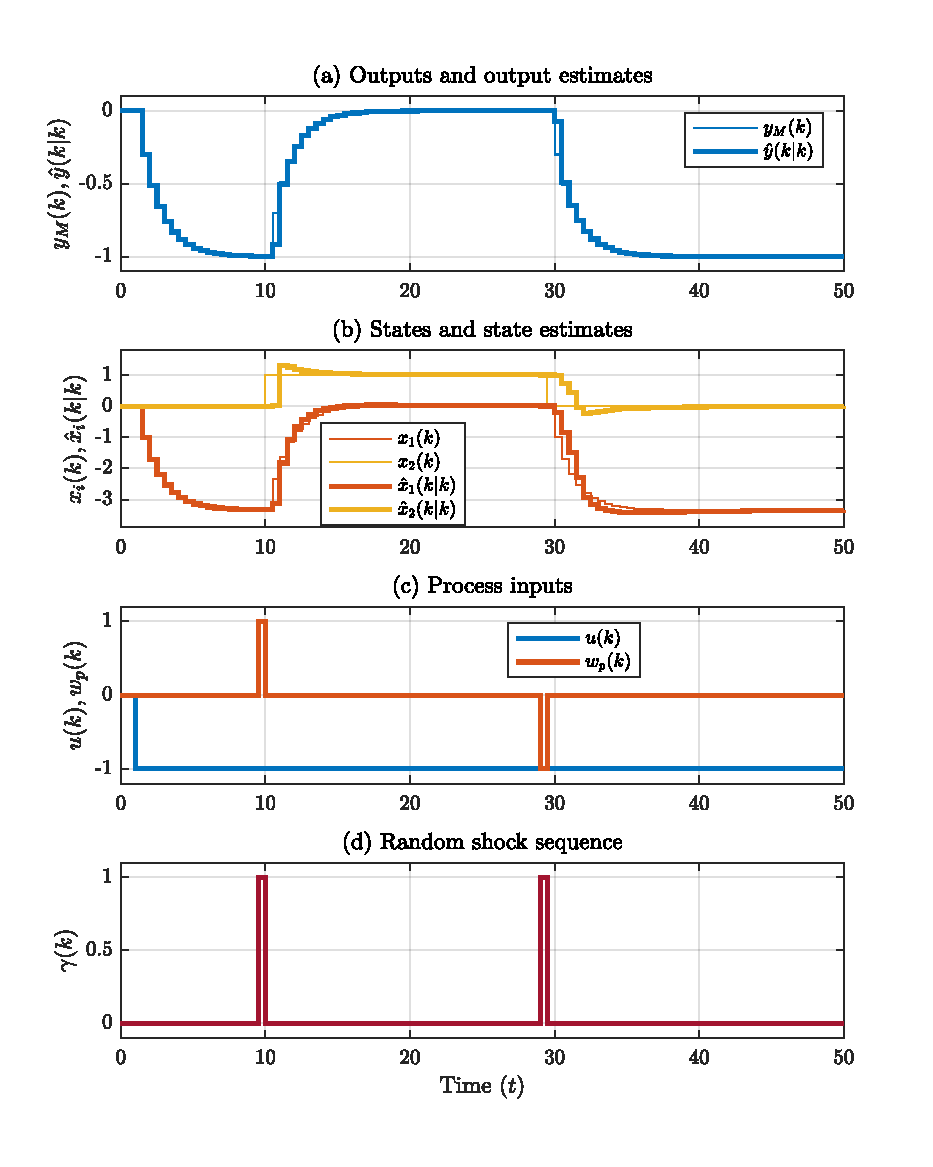
\includegraphics[width=13cm]{images/rod_MKF_SF_test_sim_MKF_SF95_ioplot.pdf}
	\caption{Simulation of a SISO linear system with a \gls{RODD} input disturbance}
	\label{fig:rod-obs-sim-test-ioplot-SF95}
\end{figure}
To understand and investigate the behaviour of the observers, the system (\ref{eq:sim-sys-siso-ss-aug}) was simulated for 100 sample periods with two pre-determined shocks, no persistent disturbance ($\sigma_{w_p}=0$), and no measurement noise ($\sigma_M=0$). Figure \ref{fig:rod-obs-sim-test-ioplot-SF95} shows the simulation data. The two lower plots show the system inputs, including the random shock signal. The upper two plots show the system states and outputs as well as the estimates of a sub-optimal multi-model observer using the sequence fusion algorithm described by \cite{robertson_detection_1995} with parameters $N_f=15$, $n_\text{max}=1$, and $N_d=5$.

\begin{figure}[htp]
	\centering
	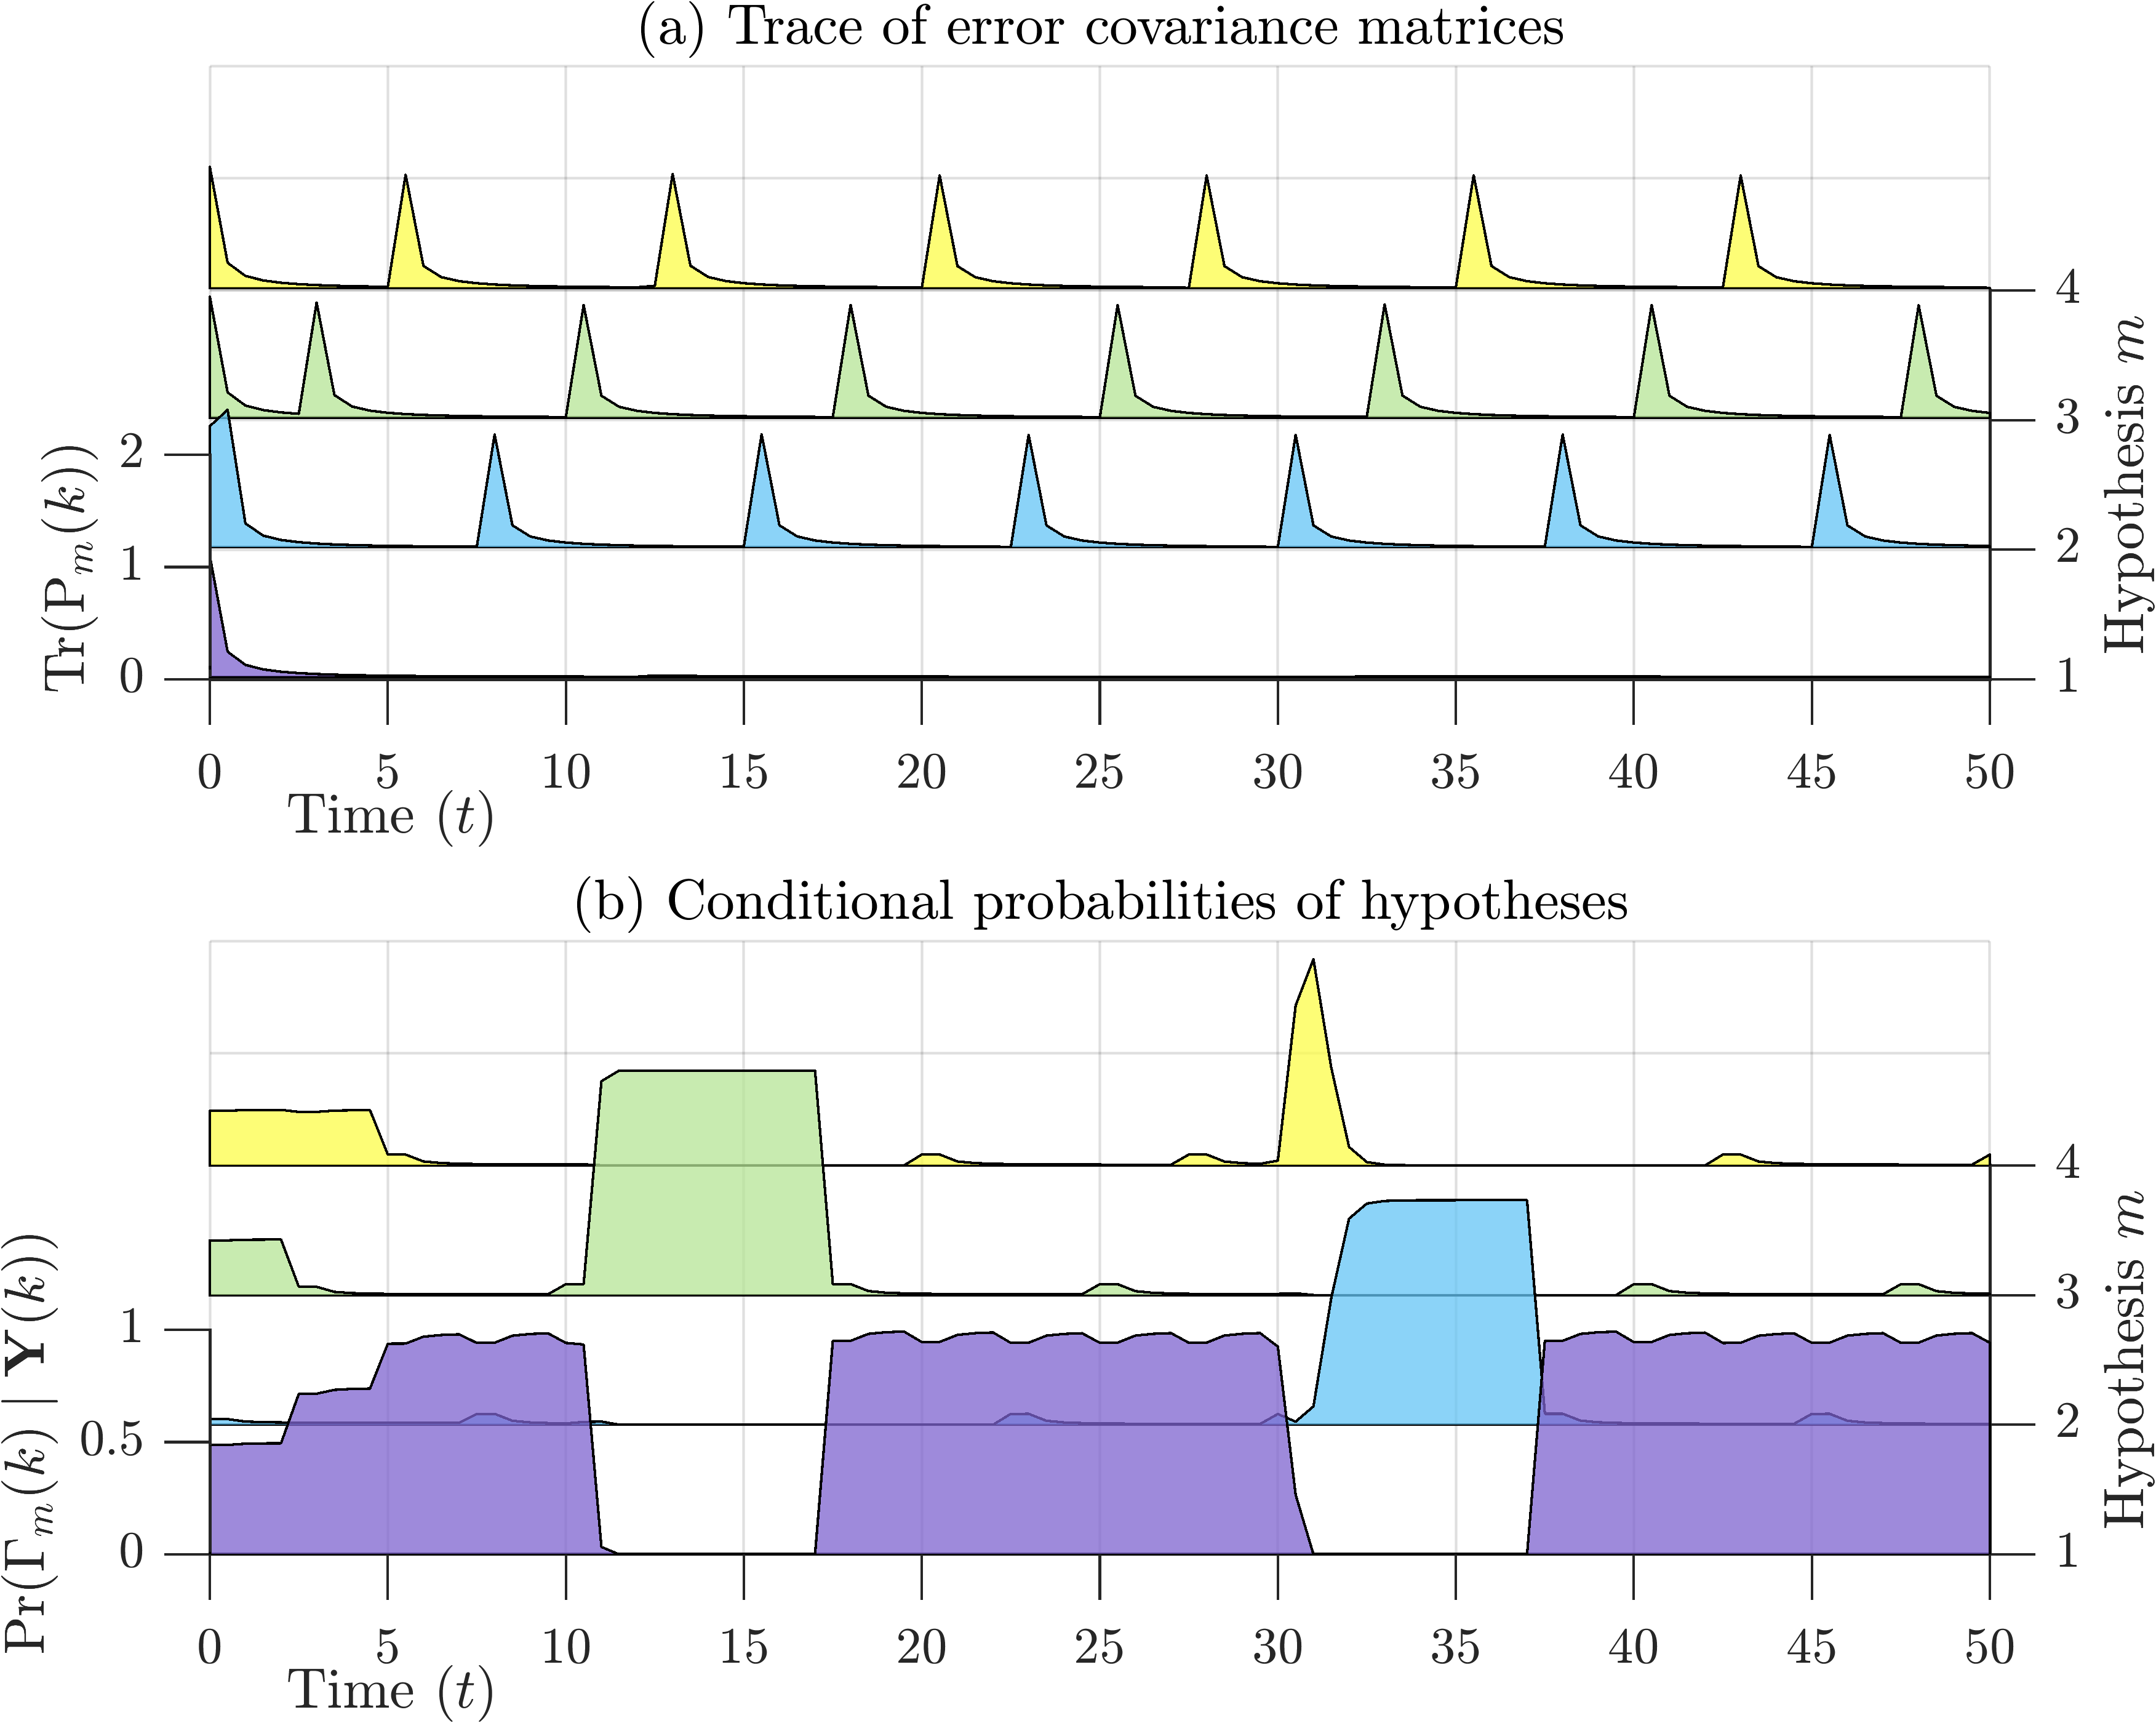
\includegraphics[width=12cm]{images/rod_MKF_test_sim_MKF_SF95_prob.png}
	\caption{Multi-model observer probability estimates – MKF--SF95}
	\label{fig:rod-obs-sim-test-probs-SF95}
\end{figure}
The two plots in Figure \ref{fig:rod-obs-sim-test-probs-SF95} provide insight into the computations of the observer, which is labelled `MKF--SF95'. The upper plot shows four time series of the trace (i.e. the sum of the elements on the main diagonal) of the merged error covariance matrices, $\mathbf{P}_m(k)$ for $m=1,2,...,n_m$. The diagonal values of $\mathbf{P}_m(k)$ may be interpreted as indicators of the magnitude of the errors of the state estimates. Recall that $\mathbf{P}_m(k)$ is time-varying and influenced by the process noise covariance, $\mathcal{Q}(\gamma_f(k))$, which switches according to the hypothesis sequences (\ref{eq:Pfkp1}). In this simulation, the covariances at time $t=0$ were initialized to the identify matrix ($\mathbf{P}_m(0)=\mathbf{I}_2$). It can be seen that the trace values initially drop rapidly and tend towards zero, however, at certain times, they increase sharply to a peak before dropping again. The sharp peaks are caused by the shock hypotheses ($\gamma_m(k)=1$) of the sequences.

The lower plot shows the conditional likelihood estimates of the four hypotheses given the data up to time $k$ after the merging step( \ref{eq:xmkymk_hat_MKF}). The conditional likelihoods were initialized to equal values ($\operatorname{Pr}\left(\Gamma_m(0) \mid \mathbf{Y}(0)\right)=1/n_m$). It can be seen that the likelihoods of each hypothesis settle on a steady-state by $t=5$ and hypothesis 1 dominates the probability distribution until $t=10$. This means that the merged estimates of the observer are determined almost completely by hypothesis 1 during this period. This makes sense since hypothesis 1 represents a sequence containing no shocks, and the first shock does not occur until $t=9.5$. A short time after the first shock occurs, the probability density shifts to hypothesis sequence 3 which happens to assume a shock at $t=10$. This is evident in the upper plot where it can be seen that the error covariance of hypothesis 3 increases peaks at $t=10.5$. The probability switches from hypothesis 1 to 3 by $t=11.5$ and remains there until $t=17$ when it shifts back to hypothesis 1. This final shift can be explained by the fusion horizon, \gls{nf}, which in this case is 15 sample periods or 7.5 time units. Hypothesis 3 assumes another shock occurs at this time, which is not the case. Therefore, hypothesis 1 becomes the most likely hypothesis after that. The second shock occurs at $t=29$, which is not as favourable since it does not align well with the shocks in any of the hypothesis sequences. Initially, the likelihood switches to hypotheses 4, which assumes a shock at $t=27.5$ but then it switches to hypothesis 2, which assumes a shock at $t=30$. Again, the probability remains high until the next shock is scheduled, at which point hypothesis 1 becomes the most likely again.

\begin{figure}[htp]
	\centering
	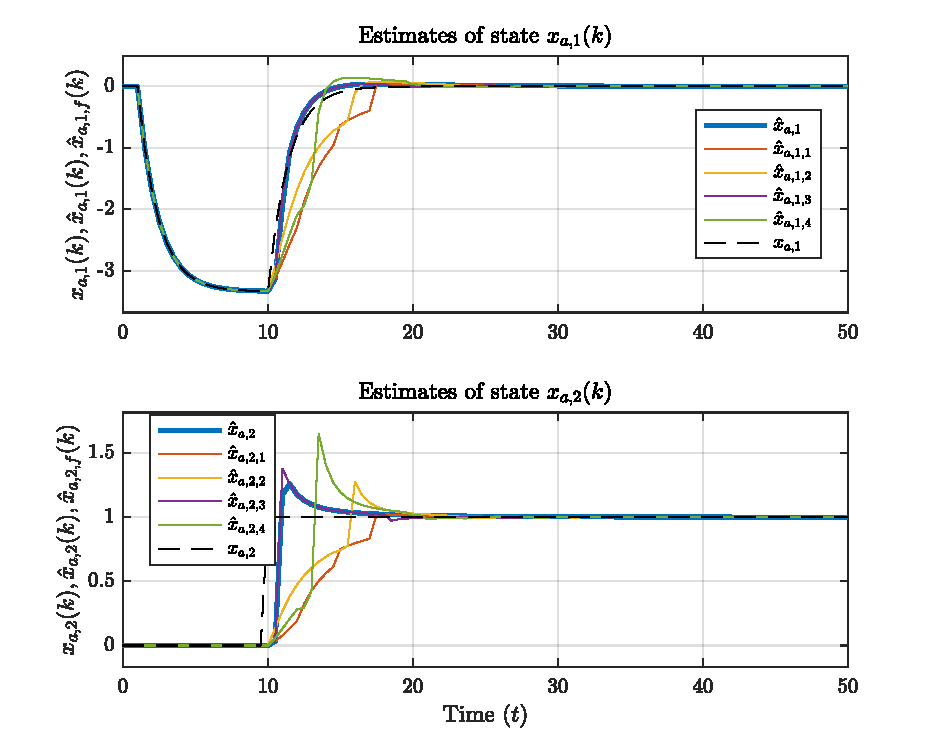
\includegraphics[width=13cm]{images/rod_MKF_test_sim_MKF_SF95_x_est.pdf}
	\caption{Multi-model observer state estimates – MKF--SF95}
	\label{fig:rod-obs-sim-test-x_est-SF95}
\end{figure}
Figure \ref{fig:rod-obs-sim-test-x_est-SF95} shows the merged state estimates associated with each hypothesis (thin coloured lines), as well as the overall state estimate (thick blue lines) and the true states of the system (dashed lines). These plots reveal the role that each hypothesis plays in the overall estimates. The estimates of hypothesis 3 (purple lines) are the first to respond to the first shock at time $t=9.5$ and the overall estimate closely follows this hypothesis. The other estimates (green, yellow and orange lines) respond at later intervals and do not play a role in the overall estimate. After the second shock occurs, the overall estimate follows that of hypothesis 2, however, this estimate lags behind the true system state and the response of the output estimate is slower and overshoots the true system output for a few time steps. These simulation results demonstrate that the performance of the sequence fusion algorithm is somewhat sensitive to the timing of the true shocks.

As described in Section \ref{subsec-fusion}, Robertson and coworkers proposed an alternative implementation of the sequence fusion algorithm in a 1998 publication. There are two differences between this and the previous algorithm. Firstly, shocks are assumed to act over the duration of the detection interval rather than at one sample time within it. Secondly, the variance of the shocks, $b^2w_{p}^2(k)$, is reduced according to the interval length, (\ref{eq:wpdk}).
%% TODO: add parameters to above? with $f=15$ $m=1$ and $d=5$.

\begin{figure}[htp]
	\centering
	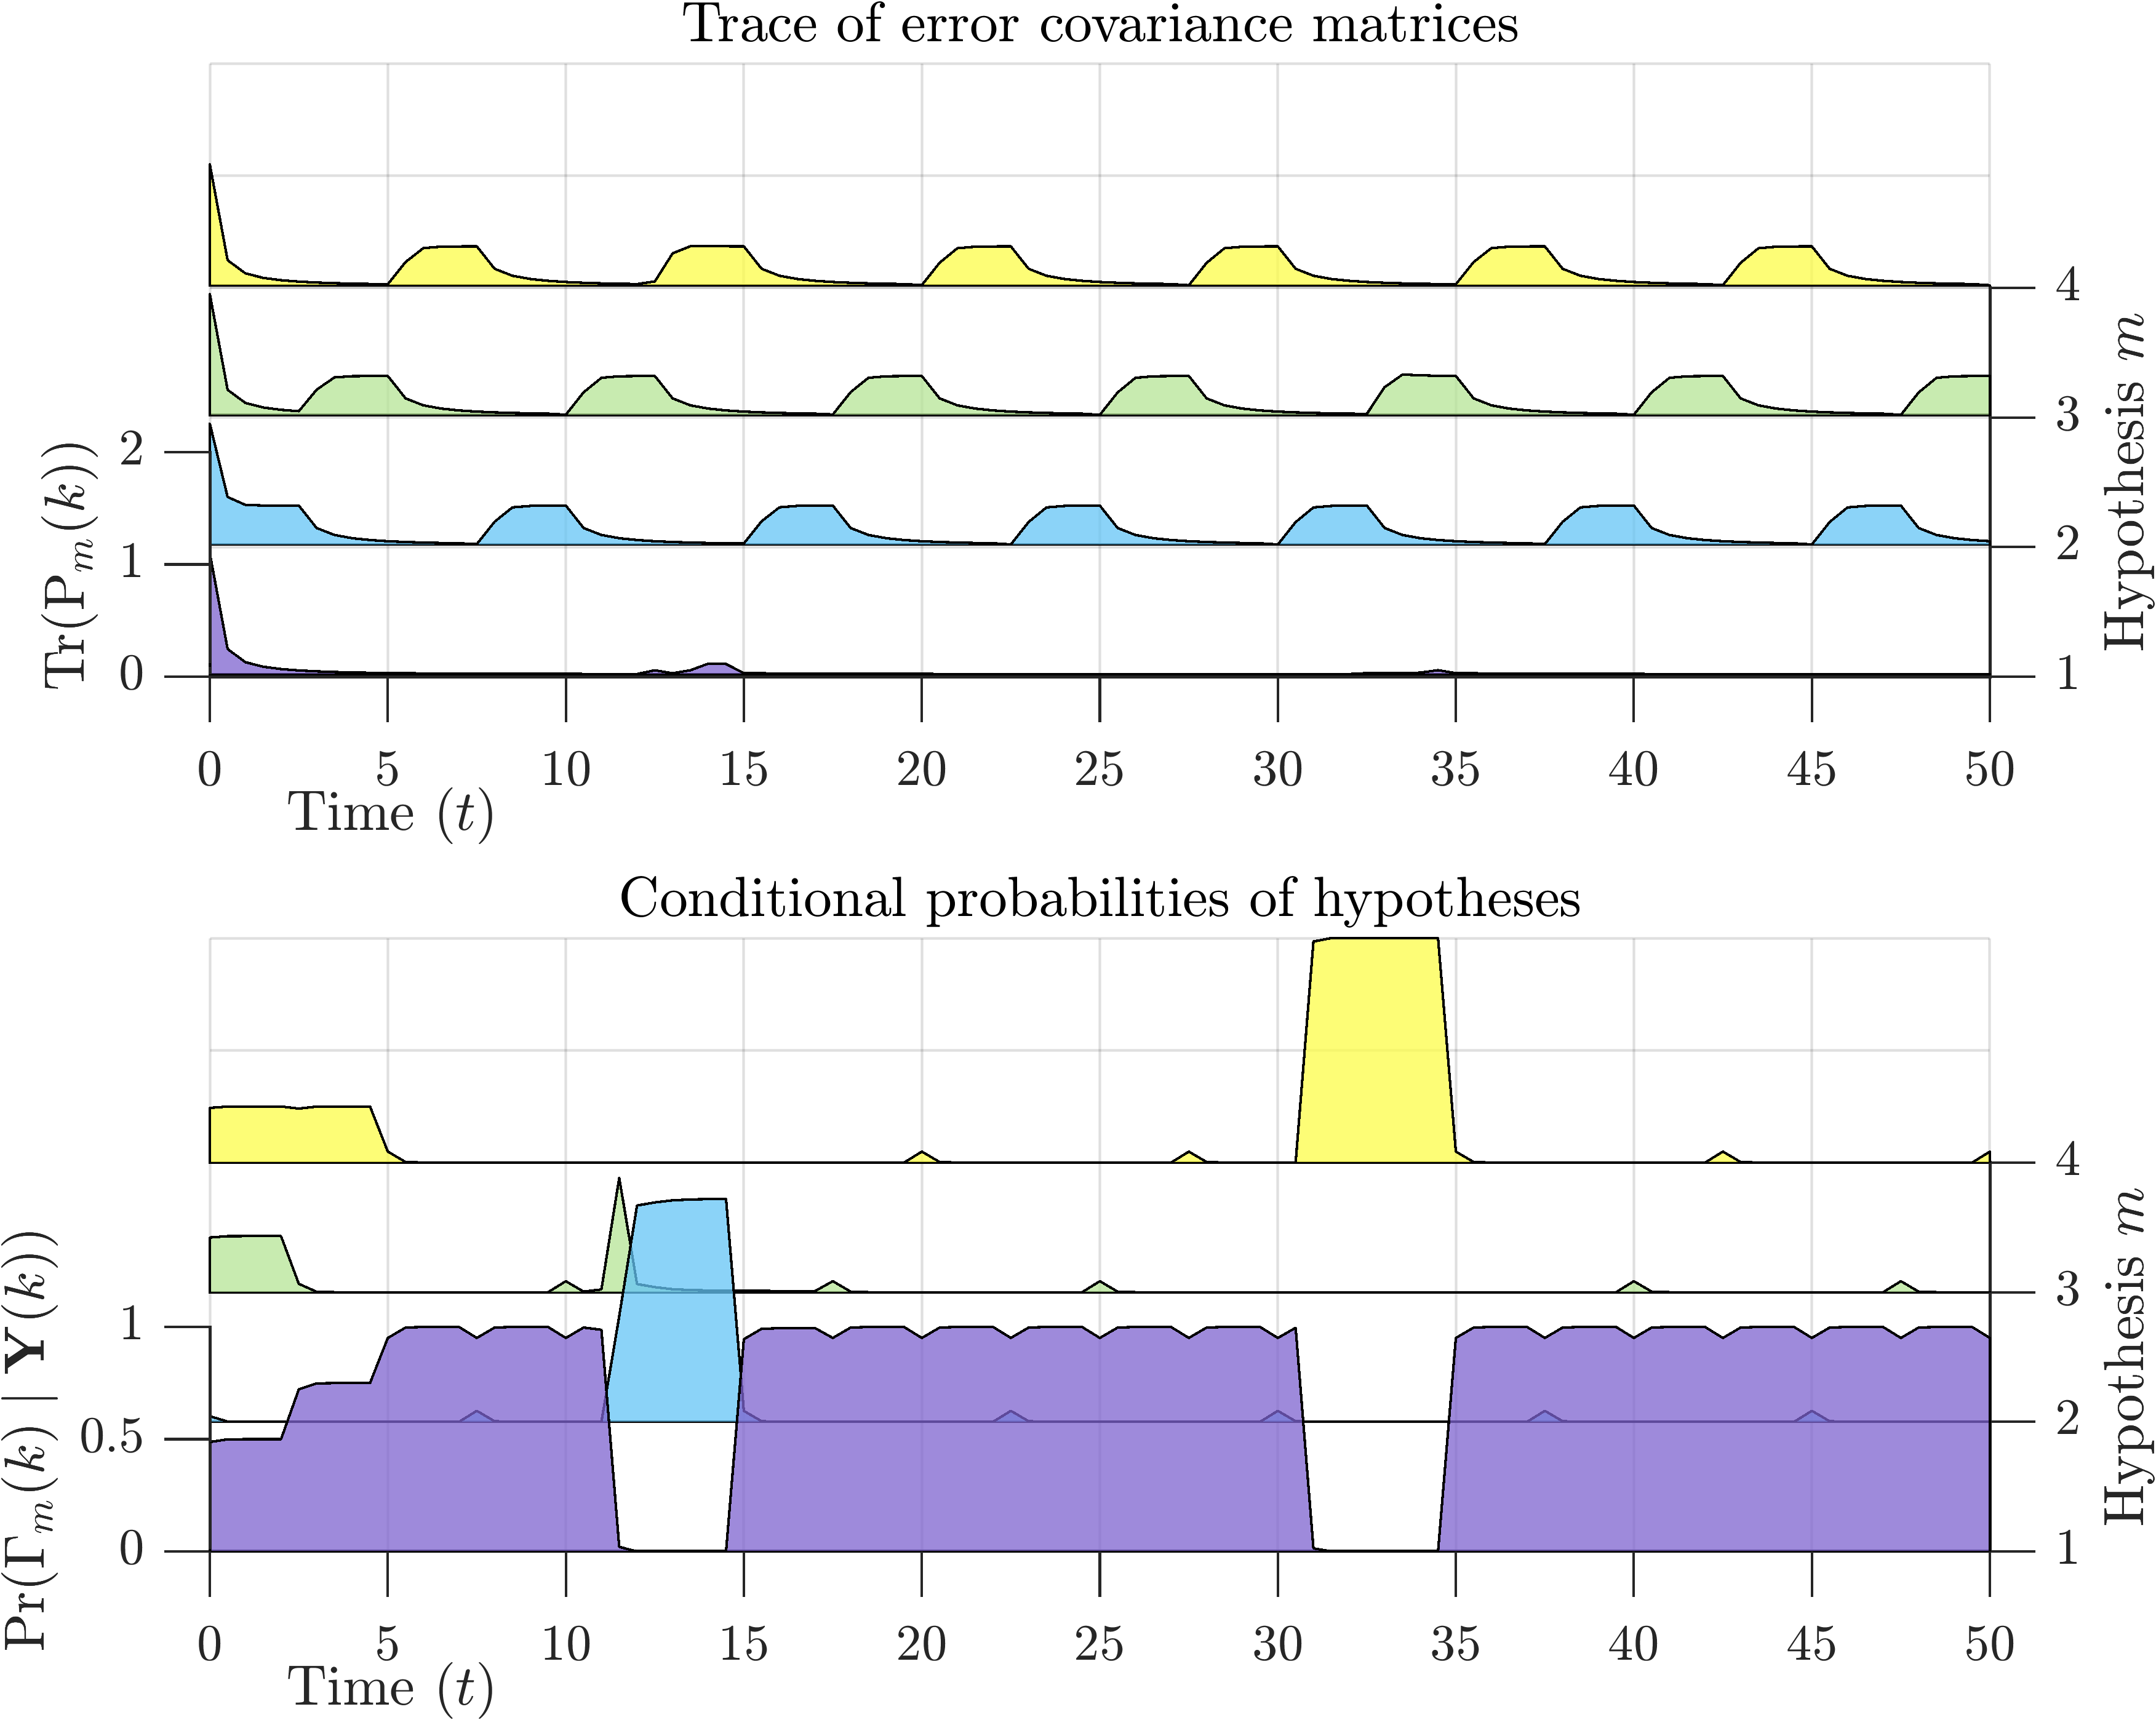
\includegraphics[width=12cm]{images/rod_MKF_test_sim_MKF_SF98_prob.png}
	\caption{Multi-model observer probability estimates – MKF--SF98}
	\label{fig:rod-obs-sim-test-probs-SF98}
\end{figure}
Figures \ref{fig:rod-obs-sim-test-probs-SF98} and \ref{fig:rod-obs-sim-test-x_est-SF98} show the results of simulating the 1998 version of the observer, labelled `MKF--SF98', with the same simulation data. The effect of the modifications on the error covariance is clear. The traces of the error covariance peak at a lower value and the peaks are sustained for the duration of the detection intervals. The switching of the hypothesis probabilities is also different. After the first shock at $t=9.5$ there is a slightly longer delay before the probability of hypothesis 3 begins to respond. However, in this case the probability then shifts to hypothesis 2. This may be due to the fact that the shock occurred in the middle of the detection interval of hypothesis 2. After the second shock at $t=29$ the response is again slower and hypothesis 4 becomes the most probable.

Figure \ref{fig:rod-obs-sim-test-x_est-SF98} shows the merged state estimates of each hypothesis, the overall estimates, and the true system states for the 1998 version of the algorithm. The behaviour of this algorithm is quite complex. The estimates take slightly longer to begin responding to shocks but there is noticeably less overshoot of the estimates in this simulation compared to the 1995 version.   
\begin{figure}[htp]
	\centering
	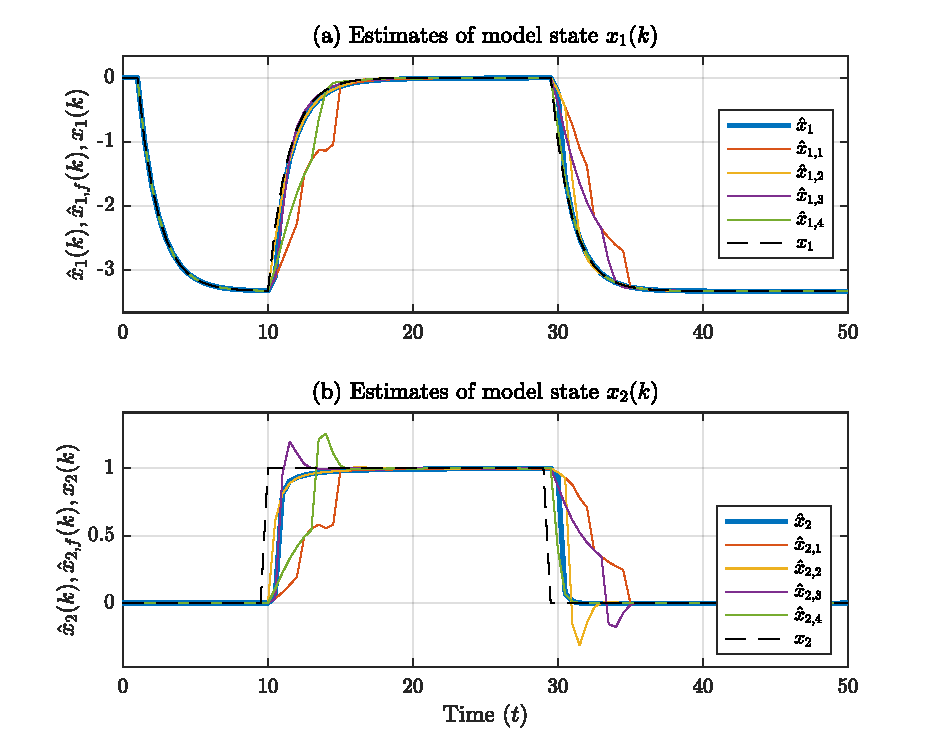
\includegraphics[width=13cm]{images/rod_MKF_test_sim_MKF_SF98_x_est.pdf}
	\caption{Multi-model observer state estimates – MKF--SF98}
	\label{fig:rod-obs-sim-test-x_est-SF98}
\end{figure}

\begin{figure}[htp]
	\centering
	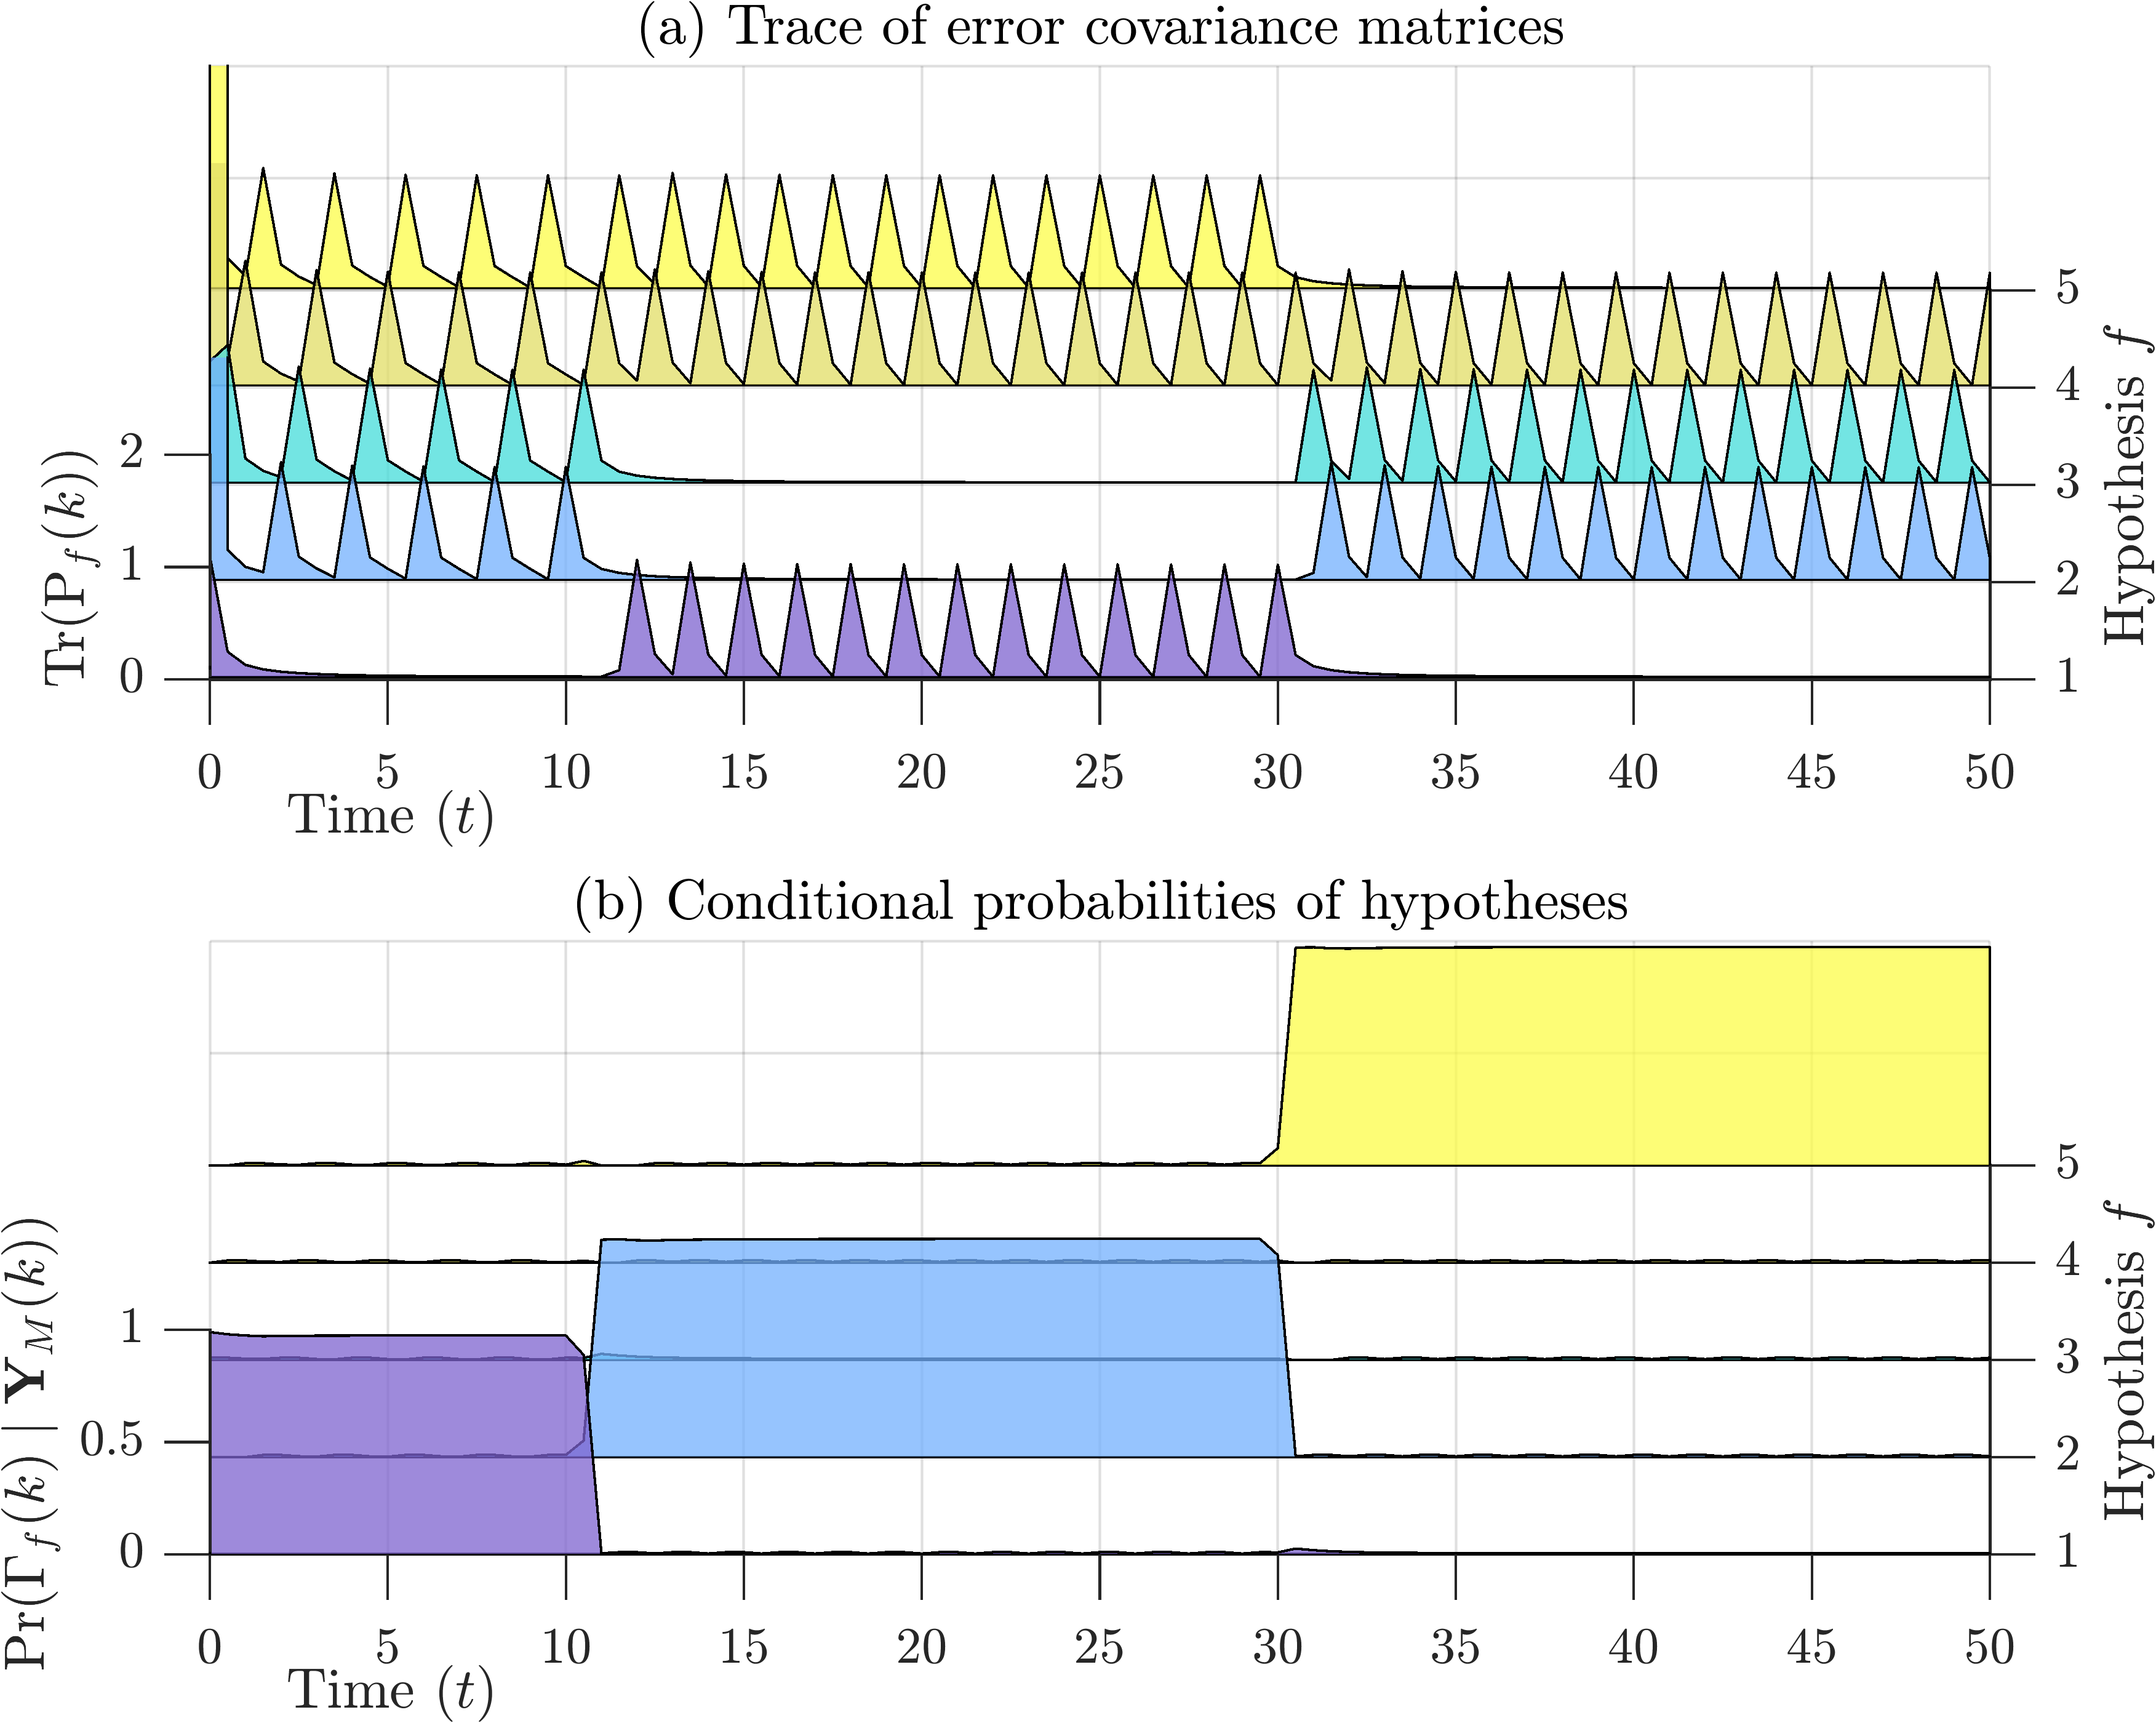
\includegraphics[width=12cm]{images/rod_MKF_test_sim_MKF_SP_prob.png}
	\caption{Multi-model observer probability estimates – MKF--SP}
	\label{fig:rod-obs-sim-test-probs-SP}
\end{figure}
\begin{figure}[htp]
	\centering
	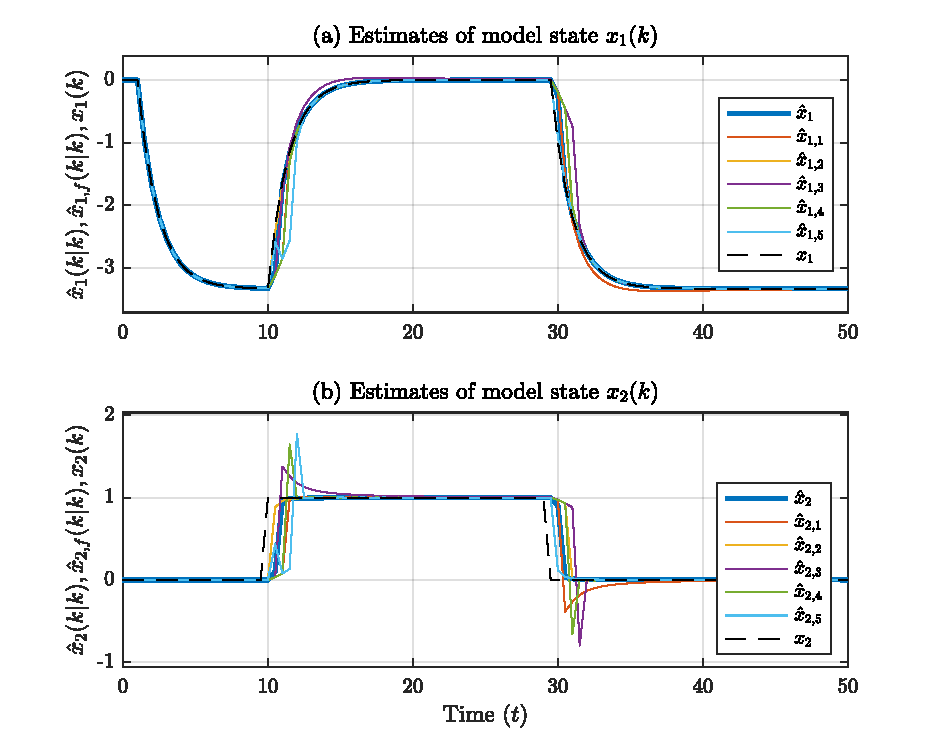
\includegraphics[width=13cm]{images/rod_MKF_test_sim_MKF_SP_x_est.pdf}
	\caption{Multi-model observer state estimates – MKF--SP}
	\label{fig:rod-obs-sim-test-x_est-SP}
\end{figure}
Figures \ref{fig:rod-obs-sim-test-probs-SP} and \ref{fig:rod-obs-sim-test-x_est-SP} show the corresponding results of simulating a sequence pruning multi-model observer (labelled `MKF--SP') with $n_h=5$ and $N_{\text{min}}=2$ as described by \cite{eriksson_classification_1996}. Recall that in this algorithm, hypotheses are adaptively pruned and replaced at every sample time. From these plots it can be seen that the hypotheses include more possible shocks than those modelled by the sequence fusion observers with detection intervals. Also, the switching of hypothesis probabilities is swifter and distinct, and the estimation errors are visibly lower than those of both versions of the sequence fusion observer in these simulations.

To effectively evaluate and compare the performance of these observers, longer simulations with pseudo-random shocks and measurement noise were used. Figure \ref{fig:rod-obs-sim1-ioplot} shows the first 600 input-output data samples from a simulation of the system with a total duration of 2500 (5000 samples). The lower plot shows the input signals, $u(k)$ and $p(k)$, from which it can be seen that two significant random shocks occurred during this period (at times $t=98$ and $220.5$). At other times, the value of $p(k)$ is a random walk due to the persistent component of the \gls{RODD} disturbance (\ref{eq:wpk2}). In addition, a step change in $u(k)$ of magnitude 1 occurred at time $t=5$. The upper plot shows the simulated output measurements. The standard deviation of the measurement noise, $\sigma_M$, was $0.1$. No disturbances other than $w_p(k)$ were simulated (i.e. $w_1(k)=0$).
\begin{figure}[htp]
	\centering
	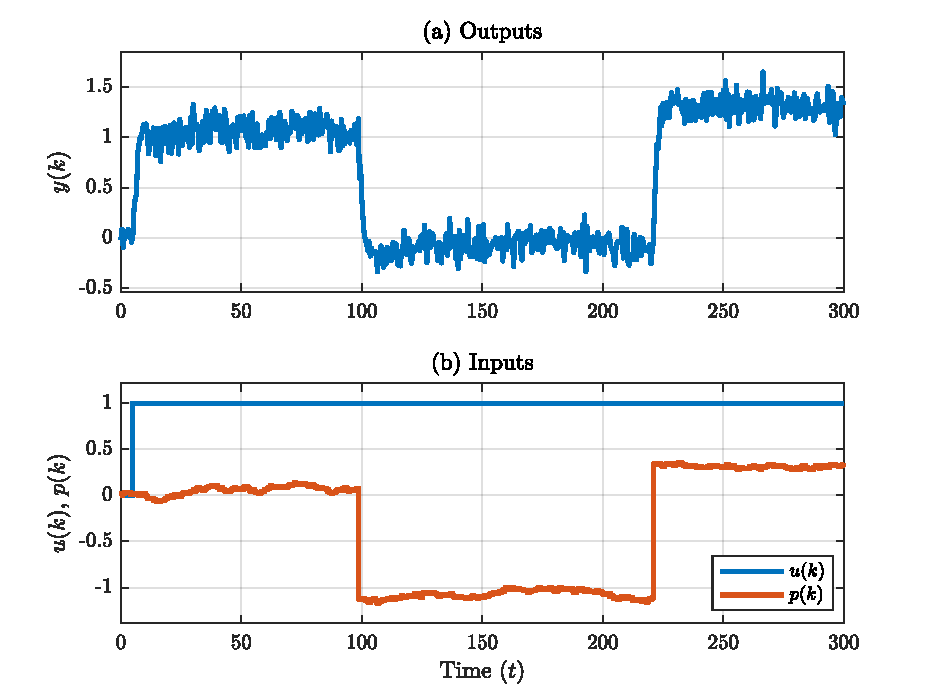
\includegraphics[width=13cm]{images/rod_obs_sim1_ioplot.pdf}
	\caption{Simulation of linear system with a \gls{RODD} input disturbance}
	\label{fig:rod-obs-sim1-ioplot}
\end{figure}

\subsubsection{Tuning of Kalman filters} \label{sim-obs-lin-1-KF-tuning}

Standard Kalman filters were used to develop performance baselines with which to evaluate the sub-optimal multi-model observers. The question of how to set the gain of a Kalman filter when there is a \gls{RODD} affecting the system is open to interpretation. One naive approach is to tune the Kalman filter using the variance of the persistent component of the disturbance, $\sigma_{w_p}^2$, if it is known. In this case, the Kalman filter, which is labelled `KF1', has a noise covariance matrix
\begin{equation} \label{eq:sim-sys-siso-KF1-Q}
	\begin{aligned}
		\mathbf{Q}_{\text{KF1}}=\mathbf{Q}_0=\begin{bmatrix}
			\sigma_{x_1}^2 & 0 \\
			0 &  \sigma_{w_p}^2 \\
		\end{bmatrix}=\begin{bmatrix}
		0.1^2 & 0 \\
		0 & 0.01^2 \\
	\end{bmatrix}
	\end{aligned},
\end{equation}
where $\sigma_{x_1}^2$ is a parameter representing the variance of the errors of the process model state, $x_1$. However, this leads to a filter with a slow response to shocks. The choice of $\sigma_{x_1}=0.1$ was a somewhat arbitrary. In these simulations, the process is simulated by a model that is identical to the model used by the observers, so there is no model error in steady-state. However, in transient periods such as after a shock disturbance, and in real applications, errors between the observer model and the true states are expected.

A second option is to tune a Kalman filter to the variance of the infrequent shocks, $b^2\sigma_{w_p}^2$.  In this case, the Kalman filter, labelled `KF2', has a state disturbance covariance matrix
\begin{equation} \label{eq:sim-sys-siso-KF2-Q}
	\begin{aligned}
		\mathbf{Q}_{\text{KF2}}=\mathbf{Q}_1=\begin{bmatrix}
			\sigma_{x_1}^2 & 0 \\
			0 & b^2\sigma_{w_p}^2 \\
		\end{bmatrix}=\begin{bmatrix}
			0.1^2 & 0 \\
			0 & 1^2 \\
		\end{bmatrix}.
	\end{aligned}
\end{equation}
The problem with this filter is that it is very sensitive to the measurement noise, $v(k)$. 

As explained by \cite{andersson_adaptive_1985} and \cite{robertson_detection_1995}, a trade-off is needed. One approach to making this trade-off is to minimize the average estimation errors over a suitably long set of input-output data. In this case, 5000 samples were generated from the simulated system (Figure \ref{fig:sim-sys-diag-siso}) and then a Kalman filter was simulated multiple times, each time with a different tuning. 
\begin{figure}[htp]
	\centering
	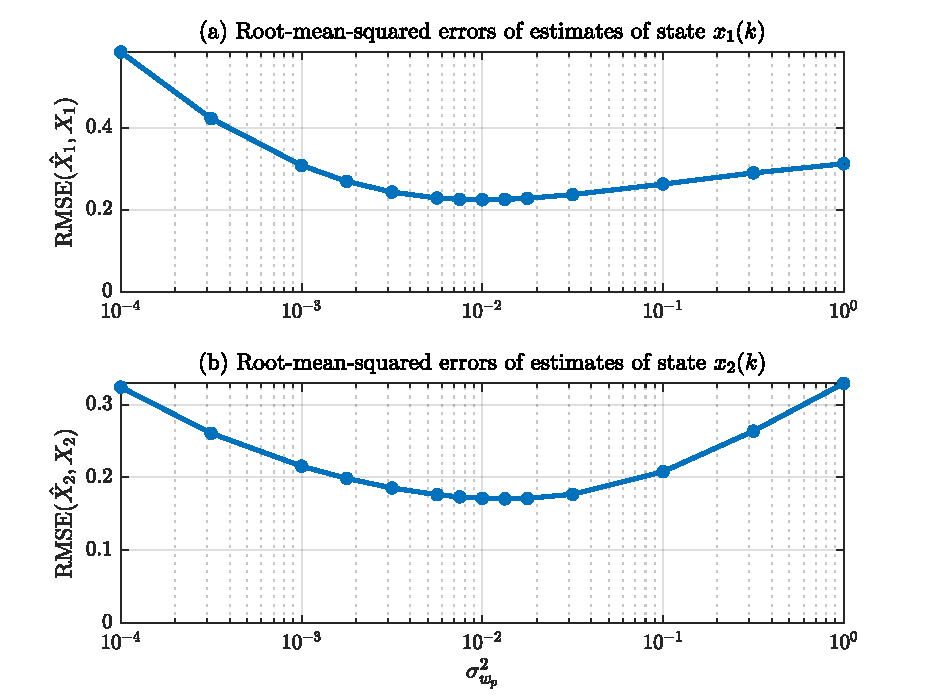
\includegraphics[width=13cm]{images/rod_obs_sim1_3KF_Q_seed_6.pdf}
	\caption{Tuning of Kalman filter KF3 – SISO system}
	\label{fig:sim-sys-siso-KF3-tuning}
\end{figure}
Figure \ref{fig:sim-sys-siso-KF3-tuning} shows the results of these simulations, from which it can be seen that the lowest \gls{RMSE}s were achieved when the variance parameter $\sigma_{w_p}^2$ was close to $0.01$. Using this result, a third Kalman filter labelled `KF3' was designed with the state disturbance covariance matrix 
\begin{equation} \label{eq:sim-sys-siso-KF3-Q}
	\begin{aligned}
		\mathbf{Q}_{\text{KF3}}=\mathbf{Q}_{\text{opt}}=\begin{bmatrix}
			\sigma_{x_1}^2 & 0 \\
			0 & \sigma_{w_p,\text{opt}}^2 \\
		\end{bmatrix}=\begin{bmatrix}
			0.1^2 & 0 \\
			0 & 0.1^2 \\
		\end{bmatrix}.
	\end{aligned}
\end{equation}

Figure \ref{fig:sim-sys-siso-KF123-est} shows the estimates of the three Kalman filters described above when simulated on the input-output data. The upper plot shows the output estimates and the lower plot shows the estimates of the second model state $x_{a,2}(k)$, which corresponds to the estimate of the \gls{RODD}, $p(k)$. As expected, the response of KF1 to the infrequent step disturbances is noticeably slower than that of the other two. The response of KF2 is fast, but it is sensitive to the measurement noise. KF3 is a compromise between the two—a relatively fast response to the infrequent step changes and less sensitivity to the measurement noise.
\begin{figure}[htp]
	\centering
	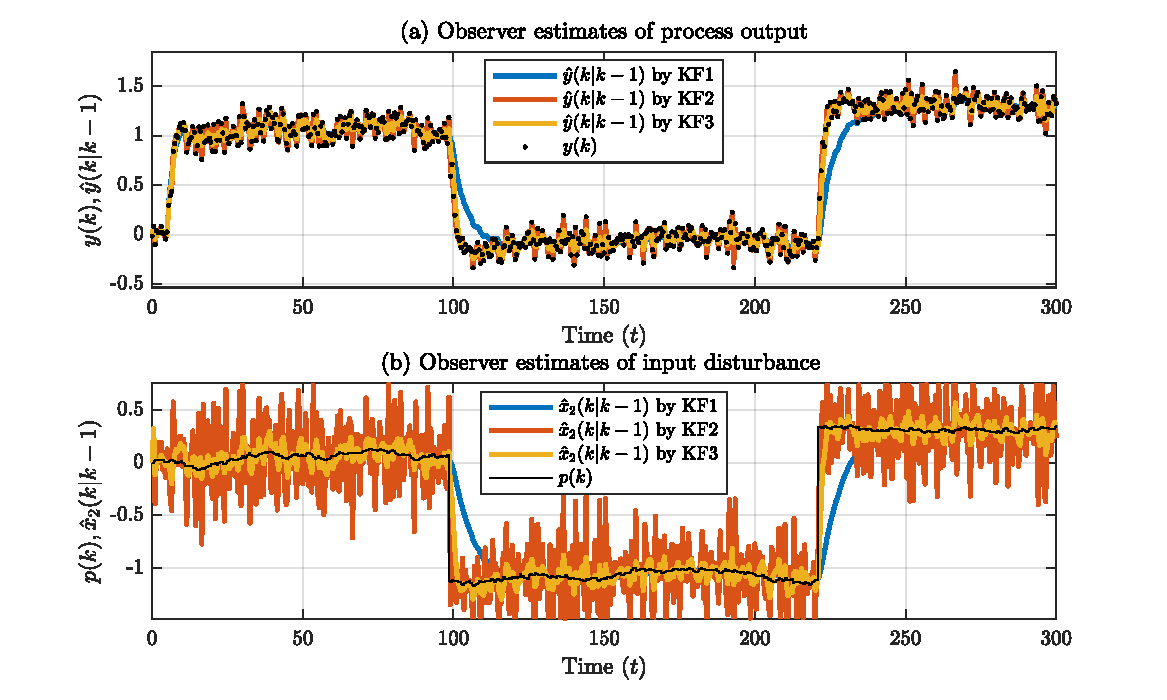
\includegraphics[width=13cm]{images/rod_obs_sim1_y_est1.pdf}
	\caption{Kalman filter estimates}
	\label {fig:sim-sys-siso-KF123-est}
\end{figure}

One way to visualise the observer performance is to plot the square of the estimation errors, which are the differences between the estimates, $\hat{y}(k \mid k)$, and the true values of the system outputs, $y(k)$. The upper plot in Figure \ref{fig:sim-sys-siso-KF123-cumerr} shows the squared errors in the output estimates of each Kalman filter. The lower plot shows the cumulative sum of the squared errors. This clearly shows the differences in performance. The estimation errors of KF1 are small when the system is in steady-state but increase dramatically after each step disturbance. The magnitude of the errors of KF2 during steady-state periods is high but roughly constant throughout the simulation. KF3 achieves the lowest overall cumulative sum-of-squared-errors by the end of the simulation.
\begin{figure}[htp]
	\centering
	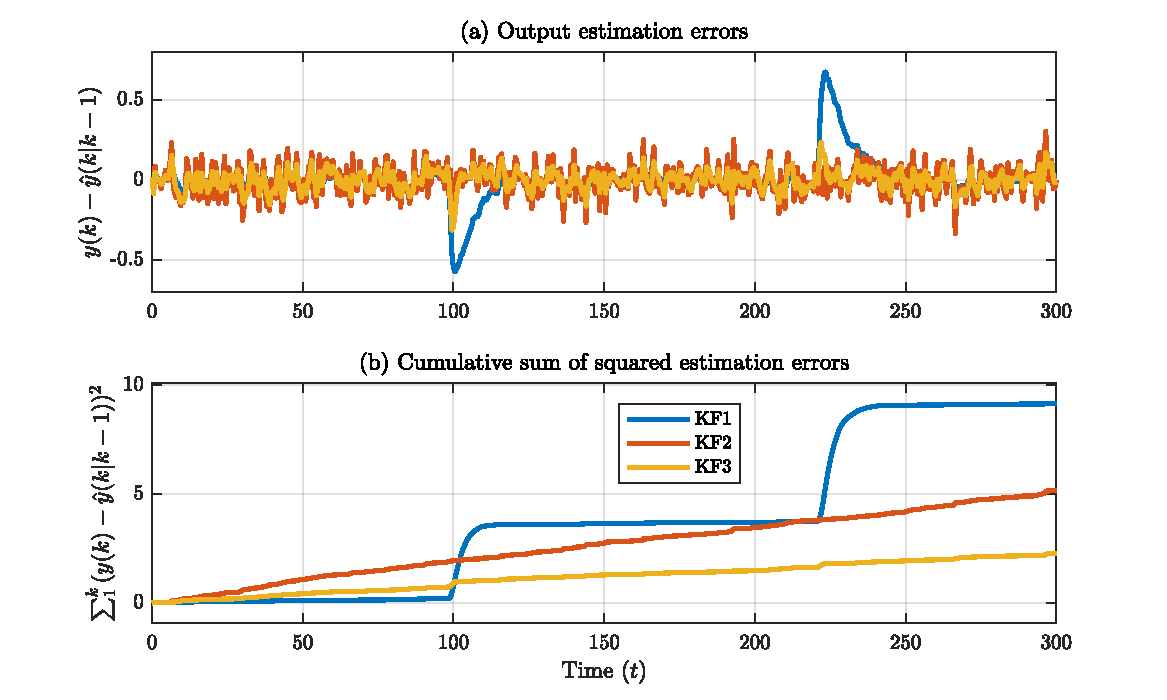
\includegraphics[width=13cm]{images/rod_obs_sim1_cum_err.pdf}
	\caption{Cumulative errors of Kalman filter estimates}
	\label{fig:sim-sys-siso-KF123-cumerr}
\end{figure}

The RMSEs of the state estimates in these simulations are shown in Figure \ref{fig:rod-obs-sim1-KF123-xest-RMSE-bar}. These plots show the total RMSEs divided into two components. The blue part, labelled `no noise' is the RMSE when the system was simulated without measurement noise, (i.e. $y_M(k)=y(k)$). The orange part, labelled `due to noise' represents the difference in the RMSE between simulating with measurement noise and without. Note that this distinction is only possible with a simulation model---in real applications it is not possible to run the system without measurement noise.
\begin{figure}[htp]
	\centering
	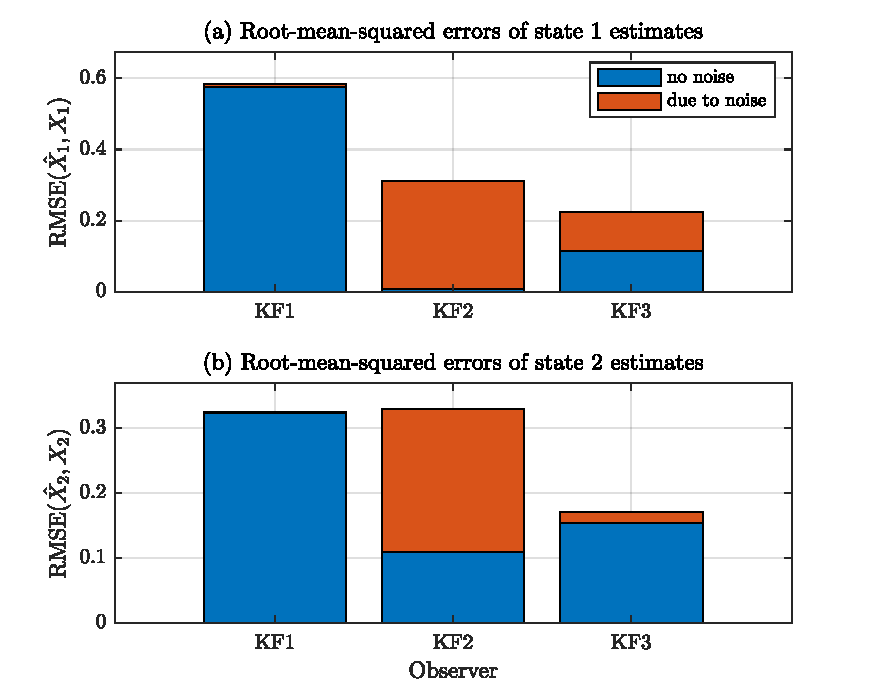
\includegraphics[width=12cm]{images/rod_obs_sim1_all_seed_x_err_bar_KF123.pdf}
	\caption{Root-mean-squared errors of state estimates – SISO system}
	\label{fig:rod-obs-sim1-KF123-xest-RMSE-bar}
\end{figure}

As well as allowing the overall RMSE values of the three Kalman filters to be compared, these plots also illustrate the relative magnitudes of the sources of the error. As expected, the errors of KF1 are almost all due to its slow dynamic response to the shocks, whereas very little is due to the measurement noise. The opposite is true of KF2, which has a very fast dynamic response to the shocks. The trade-off made between the two sources of noise is clearly illustrated for KF3. It should be noted that this is not necessarily the best trade-off in every case. In some applications, the speed of response may be more important than the sensitivity to noise, or vice-versa. However, in this work, the trade-off resulting from minimizing the overall RMSE during a long simulation is used.

\subsubsection{Selection of multi-model observer parameters} \label{sim-obs-lin-1-MKF-tuning}

Parameter values for the sub-optimal multi-model observer algorithms described in Section \ref{subsec-fusion} were chosen by a similar method. The sequence fusion algorithms proposed by \cite{robertson_detection_1995} and \cite{robertson_method_1998} have three parameters, \gls{nf}, \gls{m}, and \gls{d}. Candidate values for these parameters were generated by considering every combination satisfying

\begin{equation} \label{eq:sim-sys-siso-MKF-SF-param-values}
	\begin{aligned}
		\frac{N_f}{N_d} &\in \left\{3, 5, 10, 15, 20\right\},  \\
		n_\text{max} &\in \left\{1, 2, 3\right\},  \\
		N_d &\in \left\{1, 2, 3, 5, 10\right\}.
	\end{aligned}
\end{equation}

Note that $\frac{N_f}{N_d}$ represents the number of detection intervals within the fusion horizon and is always a whole number. For example, when $N_d=3$, the lengths of the fusion were 9, 15, 30, 45, and 60. However, not all combinations were simulated. Any combination with more than 500 hypotheses ($n_h>500$) or with a total probability modelled (\ref{eq:p_gamma}) less than 0.85 was rejected. The remaining 58 combinations were then evaluated by simulating the observer and calculating the \gls{RMSE} of the output estimates on the 5000 data samples from the simulated system. Tables \ref{tb:obs-sim1-popt-SF95} and \ref{tb:obs-sim1-popt-SF98} show the resulting \gls{RMSE} results for the 10 best combinations of parameter values (those with the lowest output \gls{RMSE}) for the 1995 and 1998 variants of this algorithm.

\begin{table}[hb]
	\begin{center}
		\caption{Multi-model observer parameter search results – MKF--SF95.} \label{tb:obs-sim1-popt-SF95}
		% See: https://texblog.org/2019/06/03/control-the-width-of-table-columns-tabular-in-latex/
		\begin{tabular}{p{0.05\textwidth}>{\centering\arraybackslash}p{0.07\textwidth}>{\centering\arraybackslash}p{0.07\textwidth}>{\centering\arraybackslash}p{0.07\textwidth}>{\centering\arraybackslash}p{0.07\textwidth}>{\centering\arraybackslash}p{0.24\textwidth}}
			$N_f$ & $n_\text{max}$ & $N_d$ & $n_h$ & $\beta$ & $\text{\gls{RMSE}}(\hat{Y}(N),Y(N))$  \\
			\hline
			% See script rod_obs_sim1_MKF_SF95_popt_table.m
			% 29-Nov-2022 18:35:37 results with seed = 6, sigma_M = 0.1, d_min = 1
			15 &   2 &   1 & 151 & 0.9996 & 0.0411 \\
			20 &   2 &   1 & 251 & 0.9990 & 0.0411 \\
			10 &   2 &   1 &  76 & 0.9999 & 0.0411 \\
			10 &   3 &   1 & 268 & 1.0000 & 0.0411 \\
			5 &   1 &   1 &   8 & 0.9990 & 0.0415 \\
			5 &   2 &   1 &  26 & 1.0000 & 0.0415 \\
			5 &   3 &   1 &  48 & 1.0000 & 0.0415 \\
			15 &   1 &   1 &  18 & 0.9904 & 0.0418 \\
			10 &   1 &   1 &  13 & 0.9957 & 0.0419 \\
			10 &   2 &   2 &  16 & 0.9043 & 0.0426 \\
			\hline
		\end{tabular}
	\end{center}
\end{table}

\begin{table}[hb]
	\begin{center}
		\caption{Multi-model observer parameter search results – MKF--SF98.} \label{tb:obs-sim1-popt-SF98}
		% See: https://texblog.org/2019/06/03/control-the-width-of-table-columns-tabular-in-latex/
		\begin{tabular}{p{0.05\textwidth}>{\centering\arraybackslash}p{0.07\textwidth}>{\centering\arraybackslash}p{0.07\textwidth}>{\centering\arraybackslash}p{0.07\textwidth}>{\centering\arraybackslash}p{0.07\textwidth}>{\centering\arraybackslash}p{0.24\textwidth}}
			$N_f$ & $n_\text{max}$ & $N_d$ & $n_h$ & $\beta$ & $\text{\gls{RMSE}}(\hat{Y}(N),Y(N))$  \\
			\hline
			% See script rod_obs_sim1_MKF_SF98_popt_table
			% 29-Nov-2022 18:38:45 results with seed = 6, sigma_M = 0.1, d_min = 1
			15 &   2 &   1 & 151 & 0.9996 & 0.0411 \\
			20 &   2 &   1 & 251 & 0.9990 & 0.0411 \\
			10 &   2 &   1 &  76 & 0.9999 & 0.0411 \\
			10 &   3 &   1 & 268 & 1.0000 & 0.0411 \\
			5 &   1 &   1 &   8 & 0.9990 & 0.0415 \\
			5 &   2 &   1 &  26 & 1.0000 & 0.0415 \\
			5 &   3 &   1 &  48 & 1.0000 & 0.0415 \\
			15 &   1 &   1 &  18 & 0.9904 & 0.0418 \\
			10 &   1 &   1 &  13 & 0.9957 & 0.0419 \\
			20 &   1 &   1 &  23 & 0.9831 & 0.0429 \\
			% Results with seed = 6, sigma_M = 0.3, d_min = 1
%			20 &   2 &   1 & 251 & 0.9990 & 0.1058 \\
%			15 &   2 &   1 & 151 & 0.9996 & 0.1059 \\
%			10 &   2 &   1 &  76 & 0.9999 & 0.1062 \\
%			10 &   3 &   1 & 268 & 1.0000 & 0.1062 \\
%			10 &   1 &   1 &  13 & 0.9957 & 0.1066 \\
%			15 &   1 &   1 &  18 & 0.9904 & 0.1070 \\
%			20 &   1 &   1 &  23 & 0.9831 & 0.1076 \\
%			5 &   1 &   1 &   8 & 0.9990 & 0.1106 \\
%			5 &   2 &   1 &  26 & 1.0000 & 0.1106 \\
%			5 &   3 &   1 &  48 & 1.0000 & 0.1106 \\
			\hline
		\end{tabular}
	\end{center}
\end{table}

In terms of overall estimation errors, both variants of the algorithm performed equally well in this simulation and the best combinations of parameter values are also the same. This can be attributed to the fact that in nearly all the top 10 combinations tested, the best value of the spacing parameter $N_d$ is 1. When $N_d=1$ there is no difference between the 1998 variant and the original algorithm. From this it may be deduced that the use of a detection interval has no benefit in this simulation scenario. \cite{robertson_method_1998} state that their approach is a means of obtaining a long detection horizon, which is necessary when many sampling intervals are required to discriminate among various abrupt changes that may occur. On this basis, it makes sense that a long detection interval was not necessary here, since the system has only one RODD.

From a practical standpoint, it is not desirable to simulate a large number of hypotheses. With this in mind, a good choice of parameters for for this system might be the third combination listed ($N_f=10,n_\text{max}=2,N_d=1$, requiring 76 hypotheses) or the fifth ($N_f=5,n_\text{max}=1,N_d=1$, requiring only 8 hypotheses). The fifth combination was chosen for for the final evaluation presented below in which the observer is labelled `MKF--SF95'. No `MKF--SF98' observer was simulated, since it provided no performance improvement over the 1995 version in this case.

The sequence pruning algorithm proposed by \cite{eriksson_classification_1996} has two parameters that must be specified, \gls{nh}, and \gls{nmin}. Candidate values for these parameters were generated by considering all combinations satisfying

\begin{equation} \label{eq:sim-sys-siso-MKF-SP-param-values}
	\begin{aligned}
		n_h &\in \left\{3, 4, 5, 7, 10, 14, 19, 25, 32\right\},  \\
			N_\text{min} &\in \left\{1, 2, 3, 4, 5, 6, 7, 9, 12, 16, 21\right\}.
		\end{aligned}
	\end{equation}

Combinations where rejected when $n_h - N_\text{min} < 1$, or in other words, when the minimum life \gls{nmin} was greater than or equal to the number of hypotheses, \gls{nh}. This is a necessary condition since there must be enough filters to simulate the hypotheses until they are pruned. Each remaining combination was then evaluated in the same way, by calculating the \gls{RMSE} of the output estimates on the same 5000 samples used in the tuning of the sequence fusion observers described above. Table \ref{tb:obs-sim1-popt-SP} shows the top 10 combinations of parameter values in terms of lowest \gls{RMSE}.

\begin{table}[hb]
	\begin{center}
		\caption{Multi-model observer parameter search results – MKF--SP.} \label{tb:obs-sim1-popt-SP}
		% See: https://texblog.org/2019/06/03/control-the-width-of-table-columns-tabular-in-latex/
		\begin{tabular}{p{0.05\textwidth}>{\centering\arraybackslash}p{0.07\textwidth}>{\centering\arraybackslash}p{0.24\textwidth}}
			$n_h$ & $N_\text{min}$ & $\text{\gls{RMSE}}(\hat{Y}(N),Y(N))$  \\
			\hline
			% See script rod_obs_sim1_MKF_SP_popt_table.m
			% 29-Nov-2022 18:24:40 results with seed = 6, sigma_M = 0.1
			10 &   7 & 0.0409  \\
			10 &   6 & 0.0410  \\
			19 &  16 & 0.0411  \\
			14 &  12 & 0.0411  \\
			25 &  21 & 0.0411  \\
			14 &   7 & 0.0411  \\
			19 &   7 & 0.0412  \\
			19 &   6 & 0.0412  \\
			25 &  16 & 0.0412  \\
			25 &  12 & 0.0412  \\
			\hline
		\end{tabular}
	\end{center}
\end{table}

As above, the differences between the \gls{RMSE}s of the best 10 combinations are small, indicating that the choice of parameters from these combinations is not critical. The first combination($n_h=10,N_\text{min}=7$) was chosen for the observer labelled `MKF--SP1' in the evaluation below. Table \ref{tb:obs-params-sim1} contains a summary of the parameters chosen for all the observers evaluated below.

\begin{table}[hb]
	\begin{center}
		\caption{Observers parameters for SISO linear system.} \label{tb:obs-params-sim1}
		% See: https://texblog.org/2019/06/03/control-the-width-of-table-columns-tabular-in-latex/
		\begin{tabular}{p{0.16\textwidth}>{\centering\arraybackslash}p{0.1\textwidth}>{\centering\arraybackslash}p{0.16\textwidth}>{\centering\arraybackslash}p{0.16\textwidth}}
			& KF3 & MKF--SF95 & MKF--SP \\
			\hline
			Type & Kalman filter & Multi-model Kalman filter & Multi-model Kalman filter \\
			Sub-optimal algorithm & - & Sequence fusion & Sequence pruning \\
			\hline
			Parameters &  &  &  \\
			$\mathbf{Q}$ & $\mathbf{Q}_{opt}$ & $\{\mathbf{Q}_0,\mathbf{Q}_1\}$ & $\{\mathbf{Q}_0,\mathbf{Q}_1\}$ \\
			$R$ & $0.1^2$ & $0.1^2$ & $0.1^2$ \\
			$\mathbf{P}(0)$ & $\mathbf{P}_0$ & $\mathbf{P}_0$ & $\mathbf{P}_0$ \\
			\gls{nh} & 1 & 4 & 10 \\
			\gls{nf} & - & 5 & - \\
			\gls{m} & - & 1 & - \\
			\gls{d} & - & 1 & - \\
			\gls{nmin} & - & - & 7 \\
			\gls{epsilon} & - & 0.01 & 0.01 \\
			\gls{sigmawp} & - & 0.01 & 0.01 \\
			\gls{b} & - & 100 & 100 \\
			\hline
		\end{tabular}
	\end{center}
\end{table}

\subsubsection{Scheduled Kalman filter} \label{sim-obs-lin-1-SKF}

To understand the maximum performance that could be achieved by an ideal multi-model observer, a hypothetical observer that has access to the true shock indicator signal $\gamma(k)$ was simulated. This `scheduled' Kalman filter, labelled ‘SKF’, has only one shock sequence---the correct one---and therefore the process noise covariance is automatically scheduled to match the known shock signal. The SKF is hypothetical because it cannot be implemented in reality since the random shocks are not measured.

\subsubsection{Stochastic simulation results} \label{sim-obs-lin-1-results}

Figure \ref{fig:rod-obs-sim1-yest-1-SF} shows the estimates of the sequence fusion observer, MKF--SF95 compared to the scheduled Kalman Filter, SKF, over the first 300 time units of the simulation. From these results it is apparent that the estimates of sequence fusion observer are generally very close to those of the SKF. The estimates respond quickly when the random shocks occur and their variance at other times is relatively small despite the measurement noise. A few spontaneous errors of short duration are also noticeable in both the SKR and MKF--SF95 estimates at certain times.
%Figure \ref{fig:rod-obs-sim1-yest-2-SF} is a closer look at the same results in the vicinity of the first step disturbance, which occurs at $t=98$.
\begin{figure}[htp]
	\centering
	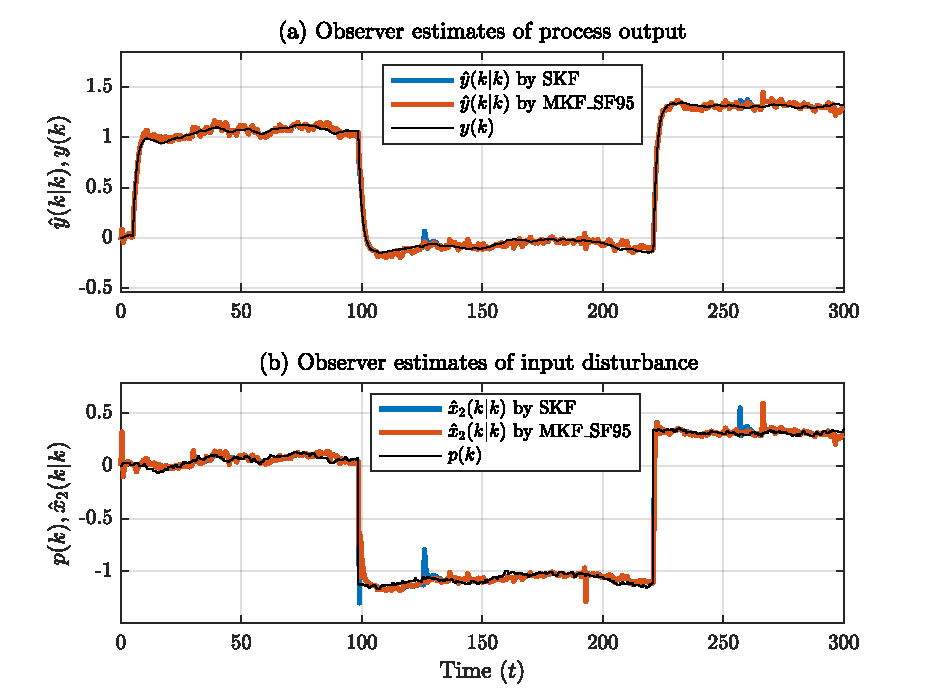
\includegraphics[width=13cm]{images/rod_obs_sim1_all_seed_y_est1_SF95.pdf}
	\caption{Estimates by sequence fusion observer – SISO system}
	\label{fig:rod-obs-sim1-yest-1-SF}
\end{figure}

% Not enough space for this detailed plot
%\begin{figure}[htp]
%	\centering
%	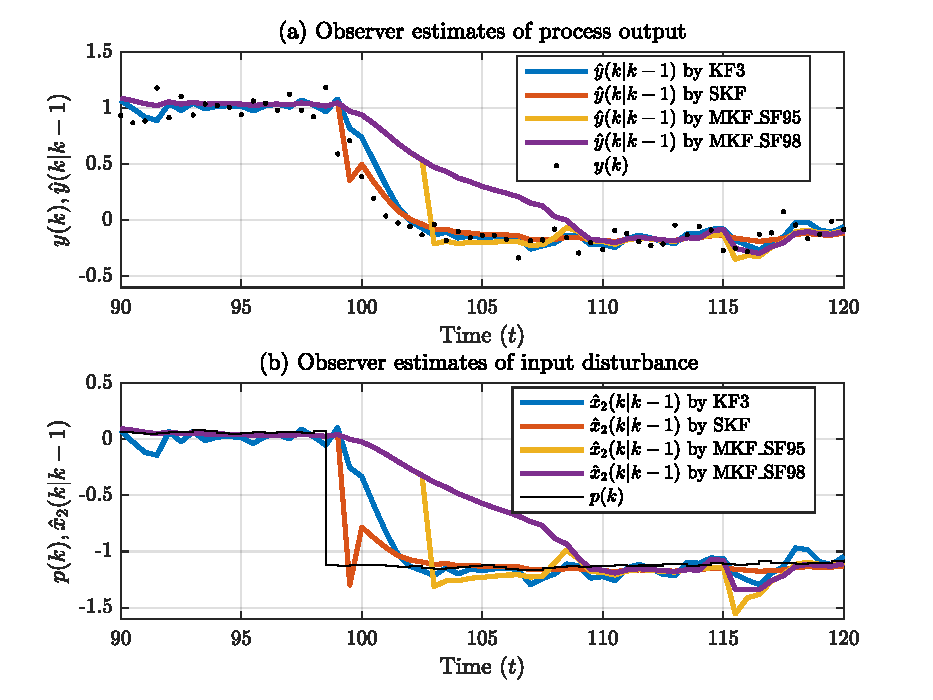
\includegraphics[width=13cm]{images/rod_obs_sim1_all_seed_y_est2_SF95_SF98.pdf}
%	\caption{Estimates by sequence fusion observer – SISO system}
%	\label{fig:rod-obs-sim1-yest-2-SF}
%\end{figure}

Figure \ref{fig:rod-obs-sim1-yest-1-SP} shows the estimates of the sequence pruning observer, MKF--SP1, compared to the scheduled Kalman Filter.  It also responds quickly to the shocks and is insensitive to the measurement noise, similar to the MKF--SF95.
\begin{figure}[htp]
	\centering
	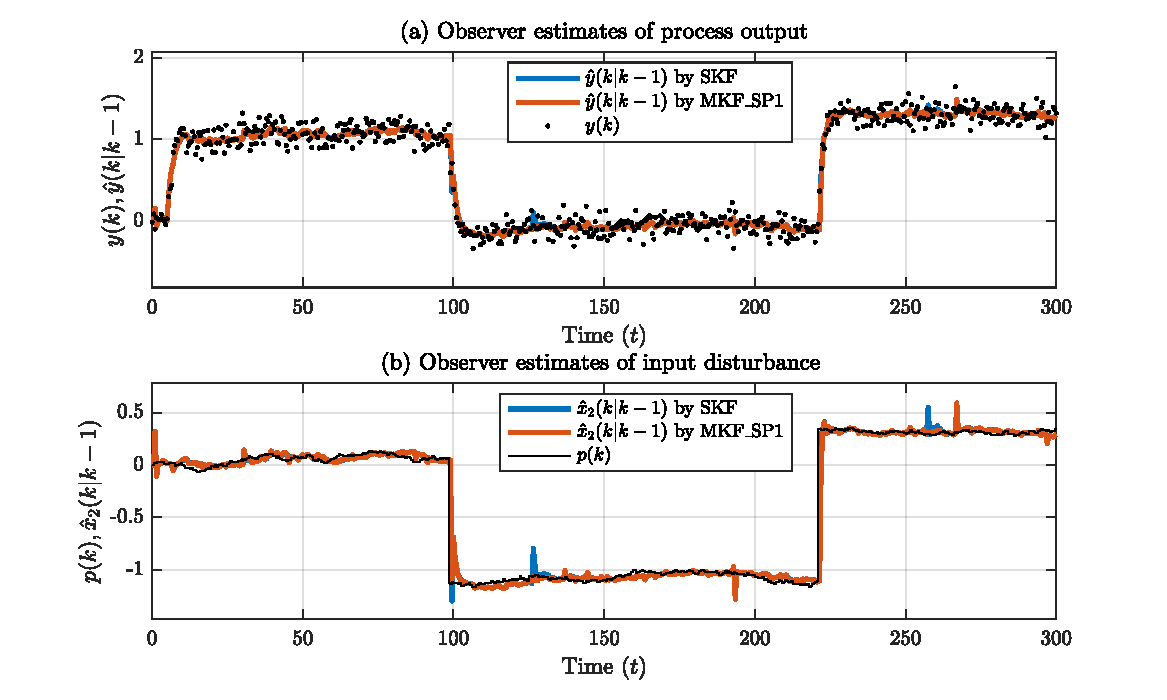
\includegraphics[width=13cm]{images/rod_obs_sim1_all_seed_y_est1_SP1.pdf}
	\caption{Estimates by sequence pruning observer – SISO system}
	\label{fig:rod-obs-sim1-yest-1-SP}
\end{figure}

% Not enough space for this detailed plot
%\begin{figure}[htp]
%	\centering
%	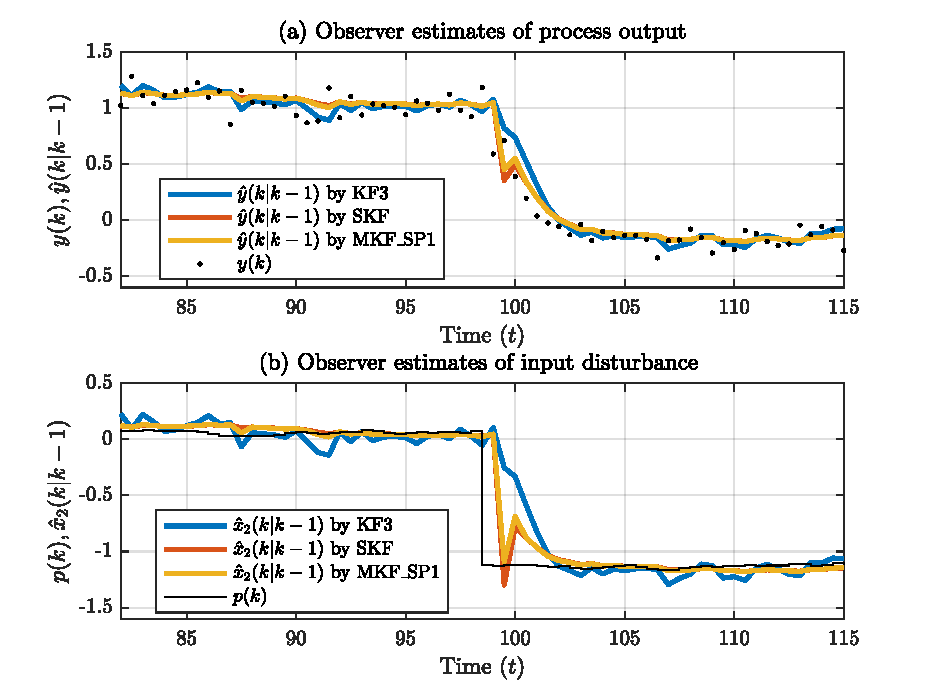
\includegraphics[width=13cm]{images/rod_obs_sim1_all_seed_y_est2_SP1.pdf}
%	\caption{Estimates by sequence pruning observer – SISO system}
%	\label{fig:rod-obs-sim1-yest-2-SP}
%\end{figure}

The plots in Figure \ref{fig:rod-obs-sim1-cum-err-y1-all} compare the output errors and the cumulative squared-errors of both multiple-model observers.
\begin{figure}[htp]
	\centering
	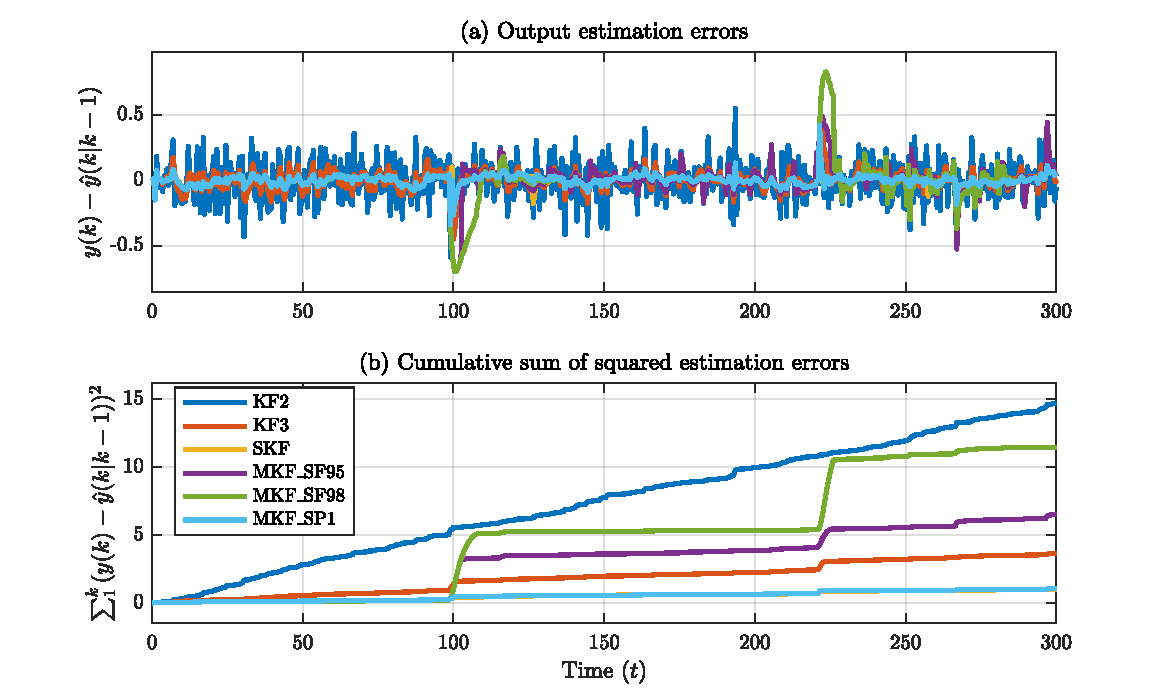
\includegraphics[width=13cm]{images/rod_obs_sim1_all_seed_cum_err_y1.pdf}
	\caption{Cumulative errors of observer estimates – SISO system}
	\label{fig:rod-obs-sim1-cum-err-y1-all}
\end{figure}

Figure \ref{fig:rod-obs-sim1-xest-RMSE-bar} compares the \gls{RMSE}s of the state estimates of the five observers over the full length of the simulation, (total duration 2500, or 5000 sample periods). This confirms that the multiple-model observers produced better estimates on average than either of the standard Kalman filters and almost as good as those of the SKF.
\begin{figure}[htp]
	\centering
	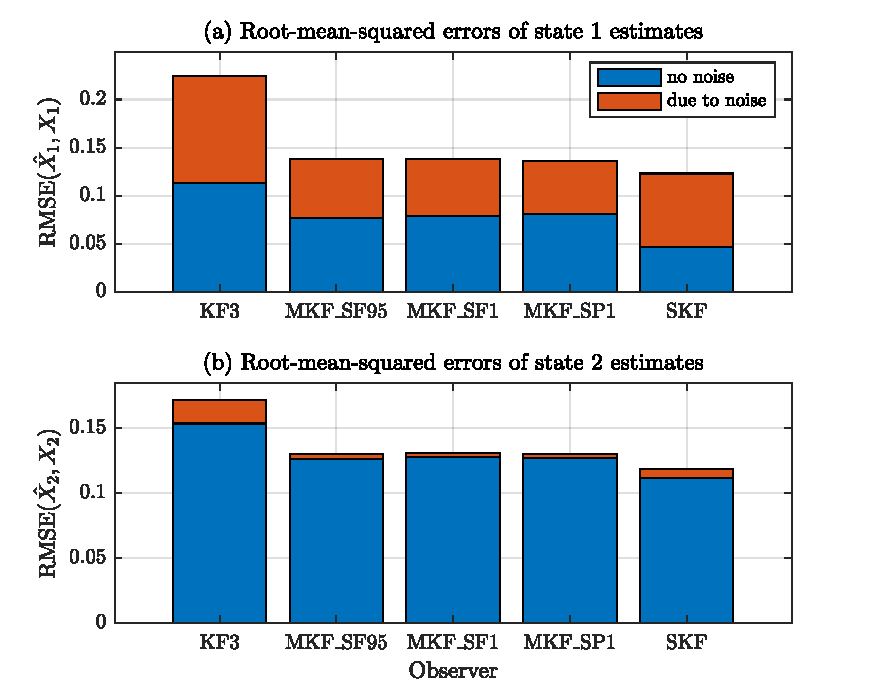
\includegraphics[width=12cm]{images/rod_obs_sim1_all_seed_x_err_bar.pdf}
	\caption{Root-mean-squared errors of state estimates – SISO system}
	\label{fig:rod-obs-sim1-xest-RMSE-bar}
\end{figure}

Because these processes are stochastic, it is important to run simulations of sufficient duration to be confident that the results are representative of the expected performance of the observers. Figure \ref{fig:rod-obs-sim1-yest-all-seed-RMSE-box} provides an indication of the sensitivity of the \gls{RMSE} values to the initialization of the pseudo-random number generator used in these simulations. This figure shows the results of 10 simulations of 5000 samples each, carried out with different initializations. From these results it can be seen that the \gls{RMSE} values are somewhat sensitive to the random initialization but that the differences between the three observers are significant enough and highly unlikely to be a result of the random initialization. Therefore, these simulations of duration 5000 sample periods may be considered sufficient for the purposes of evaluating the relative performance of these observers.
\begin{figure}[htp]
	\centering
	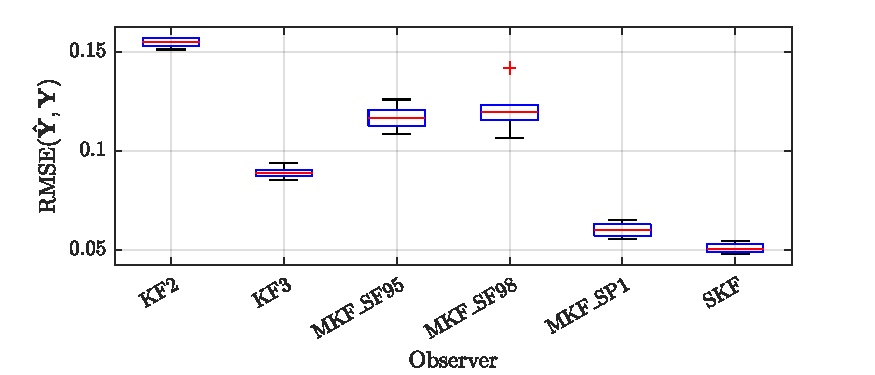
\includegraphics[width=12cm]{images/rod_obs_sim1_all_seed_y_err_box.pdf}
	\caption{Sensitivity of output estimation errors to random initialization – SISO system}
	\label{fig:rod-obs-sim1-yest-all-seed-RMSE-box}
\end{figure}

% Plots for analysis of SF performance
%
%\begin{figure}[htp]
%	\centering
%	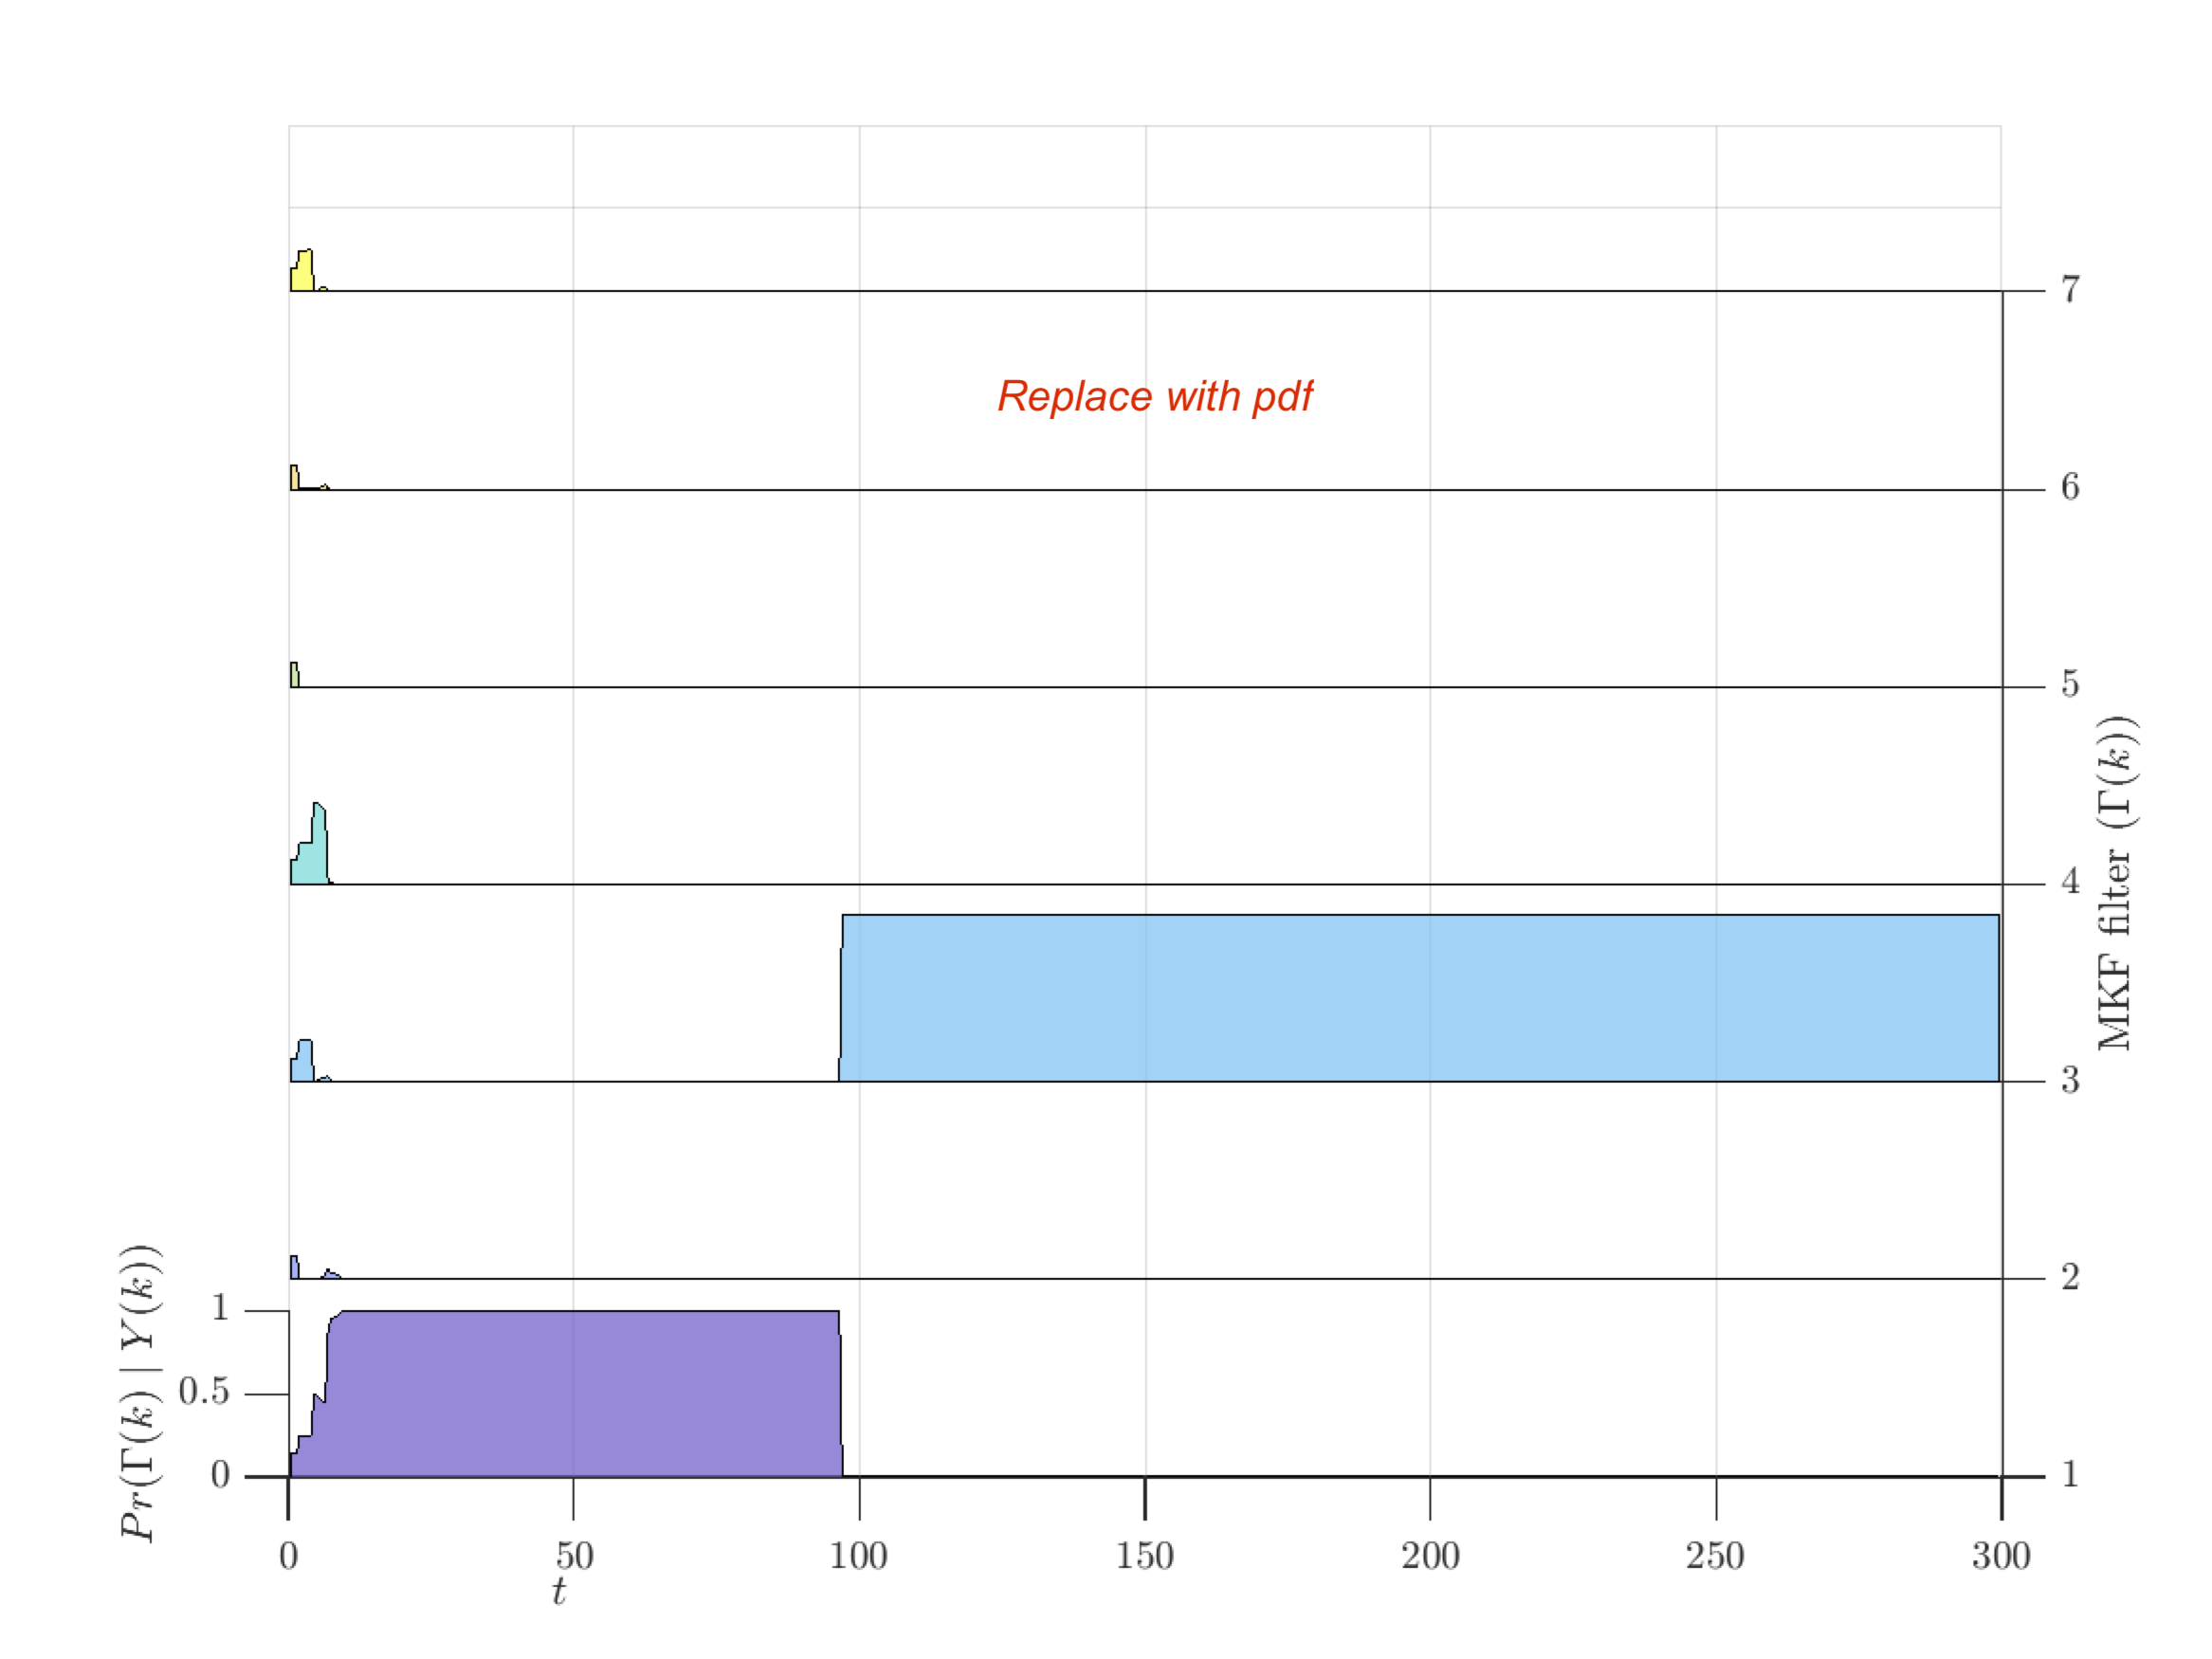
\includegraphics[width=15cm]{images/rod-obs-sim-1-4-wfplot-DRAFT.png}
%	\caption{Evolution of conditional probabilities with sequence fusion}
%	\label{fig:rod-obs-sim1-4-wfplot}
%\end{figure}
%
%\begin{figure}[htp]
%	\centering
%	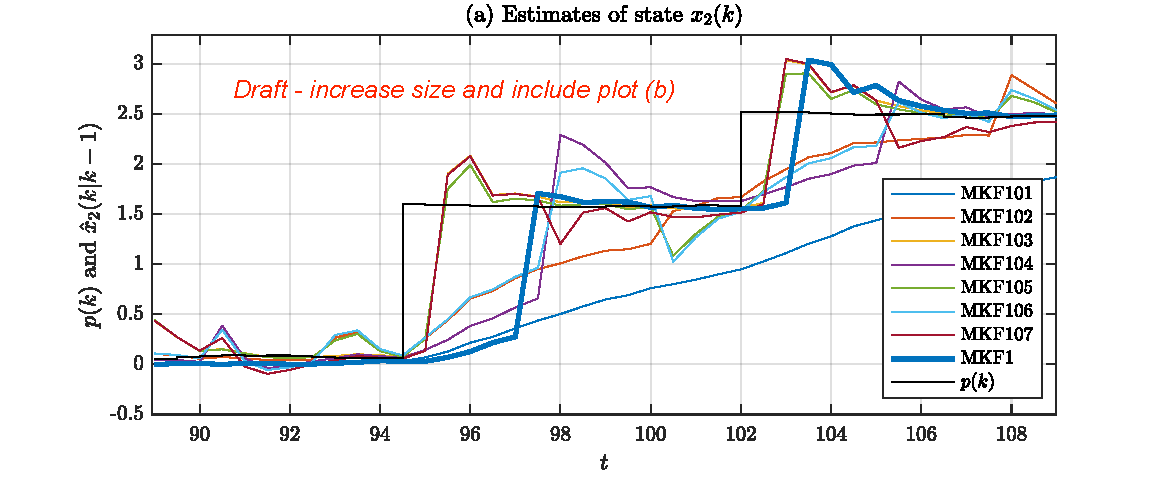
\includegraphics[width=14cm]{images/rod-obs-sim-1-4-est-MKF-SF-plot-DRAFT.pdf}
%	\caption{Filter estimates of sequence fusion observer during step disturbances}
%	\label{fig:rod-obs-sim1-4-est-MKF-SF-plot-DRAFT}
%\end{figure}
%
%\begin{figure}[htp]
%	\centering
%	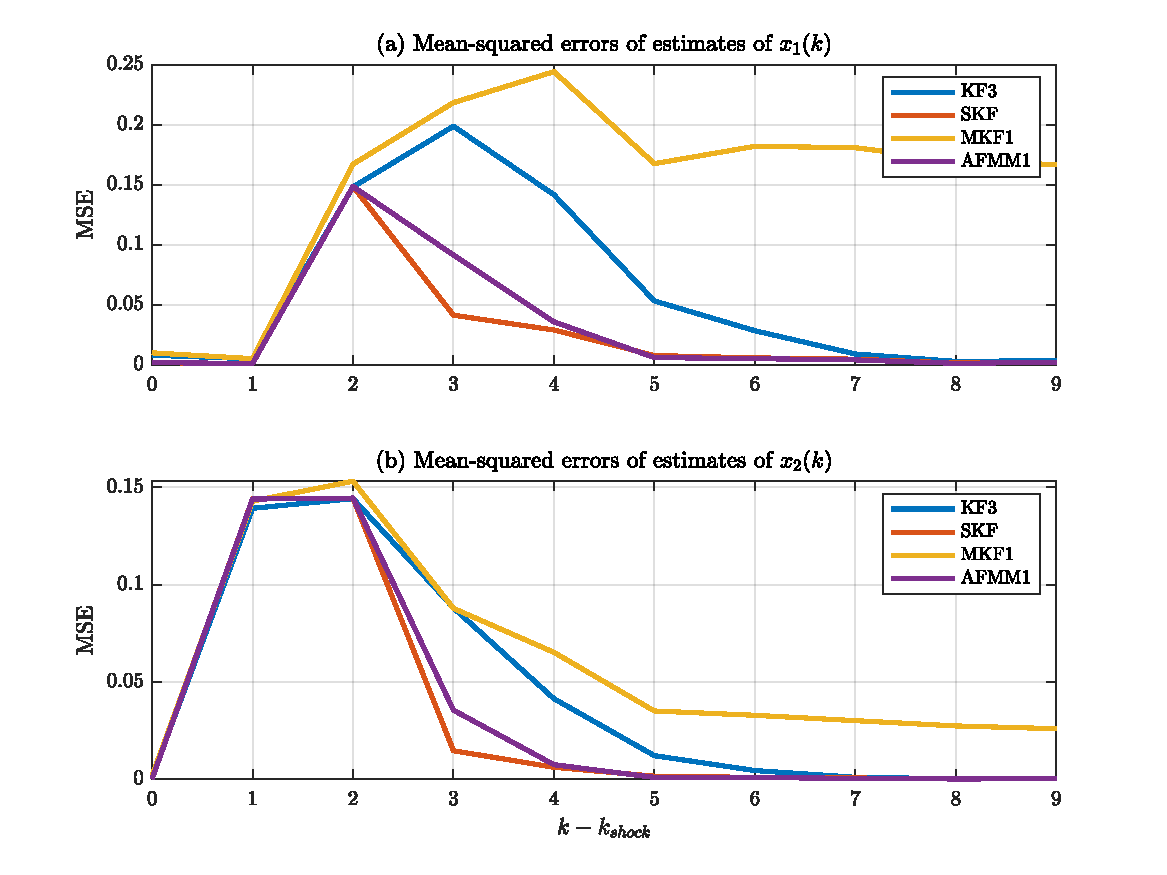
\includegraphics[width=14cm]{images/rod_obs_sim2_7_mse_ashocks.pdf}
%	\caption{Average errors of observer estimates after shock disturbances}
%	\label{fig:rod_obs_sim2_7_mse_ashocks}
%\end{figure}

\subsection{MIMO linear system} \label{sim-obs-lin-2}

To investigate the performance of the observers in estimating the states of a \textit{multiple-input, multiple output} (MIMO) system, a 2-input, 2-output ($2\times2$) process model was chosen, with two independent \gls{RODD} step disturbances added to each manipulated input, as shown in the functional diagram in Figure \ref{fig:sim-sys-diag-2x2}. 

The model used to simulate the process is a discrete-time linear model derived from the continuous-time system,
\begin{equation} \label{eq:sim-sys-siso--ct}
	\mathbf{G}_p(s) = \left[\begin{array}{cc}
		G_{11}(s) & G_{12}(s)  \\
		G_{21}(s) & G_{22}(s)  \\
	\end{array}\right] = \left[\begin{array}{cc}
		\frac{1}{1+8.5s} & \frac{-0.5}{1+8.5s}  \\
		\frac{-0.5}{1+8.5s} & \frac{1}{1+8.5s}  \\
	\end{array}\right]
\end{equation}
where $s$ is the Laplace variable.  This was converted to a discrete-time model with a sampling period of $T=1$. The discrete-time state space representation used to simulate the augmented system including disturbances was
\begin{equation} \label{eq:sim-sys-2x2-ss-aug}
	\begin{split}
		\mathbf{x}_{a}(k+1) & =\left[\begin{array}{cccc}
			0.8890 & 0 & 1 & -0.5 \\
			0 & 0.8890 & -0.5 & 1 \\
			0 & 0 & 1 & 0 \\
			0 & 0 & 0 & 1
		\end{array}\right] \mathbf{x}_{a}(k) + \left[\begin{array}{cc}
			1 & -0.5 \\
			-0.5 & 1
		\end{array}\right] \mathbf{u}(k) + \mathbf{w}_{a}(k) \\
		y(k) & =\left[\begin{array}{cccc}
			0.1110 & 0 & 0 & 0 \\
			0 & 0.1110 & 0 & 0
		\end{array}\right] \mathbf{x}_{a}(k) + v(k)
	\end{split}
\end{equation}
where
\begin{equation} \label{eq:sim-sys-2x2-ss-aug2}
	\mathbf{x}_{a}(k) = \left[\begin{array}{l}
		x_{1}(k) \\
		x_{2}(k) \\
		p_{1}(k) \\
		p_{2}(k)
	\end{array}\right], \mathbf{w}_{a}(k) = \left[\begin{array}{l}
		w_1(k) \\
		w_2(k) \\
		w_{p,1}(k) \\
		w_{p,2}(k)
	\end{array}\right].
\end{equation}

Random shocks with probabilities $\epsilon=\begin{bsmallmatrix}0.01 & 0.01\end{bsmallmatrix}^\intercal, \sigma_{wp}=0.01$, and $b=100$ were simulated. Figure \ref{fig:rod-obs-sim-2-ioplot} shows the first 600 input-output data samples from a simulation of the system with a total duration of 2500 (5000 samples). The lower of the two plots shows the input signals, $u_1(k)$, $u_2(k)$, $p_1(k)$, and $p_2(k)$. From this it can be seen that a large shock occurred to $p_1(k)$ at $t=122$ and 6 random shocks occurred to $p_2(k)$ of various magnitudes. In this simulation, there were no changes to the known input variables. The upper plot shows the simulated output measurements, $y_1(k)$ and $y_2(k)$. The standard deviation of the measurement noises, $\sigma_{M,1}$ and $\sigma_{M,2}$, were both $0.2$. No input disturbances other than $w_{p,1}(k)$ and $w_{p,2}(k)$ were simulated (i.e. $w_1(k)=w_2(k)=0$).

As in the previous experiment, a standard Kalman filter was tuned experimentally to achieve a low \gls{RMSE} of the output estimates. The details of this tuning process are included in Annex \ref{section:annex-sim-2-KF-tuning}. 
% Best KF tuning was $\sigma_{w_p}^2=0.0075$  After changing measurement noise, it is now it is 0.01.

\begin{figure}[htp]
	\centering
	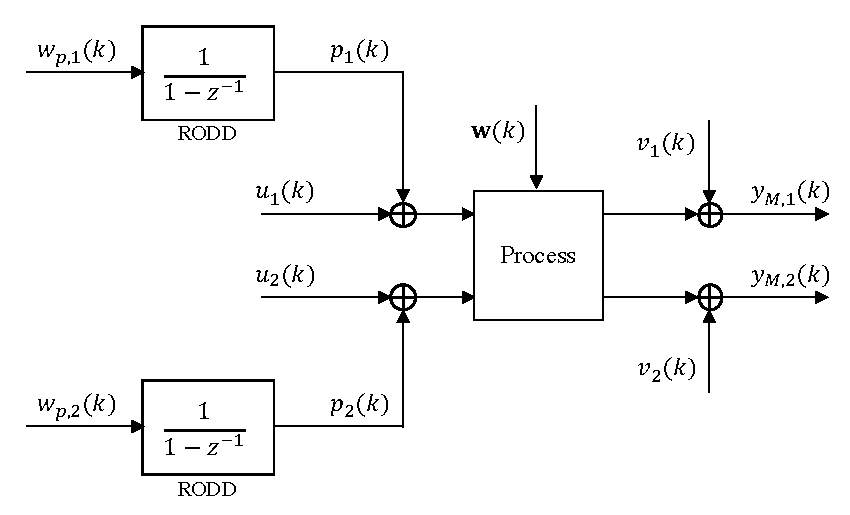
\includegraphics[width=11.5cm]{images/sim-sys-diag-2x2.pdf}
	\caption{Functional diagram of the simulated MIMO system}
	\label{fig:sim-sys-diag-2x2}
\end{figure}

\begin{figure}[htp]
	\centering
	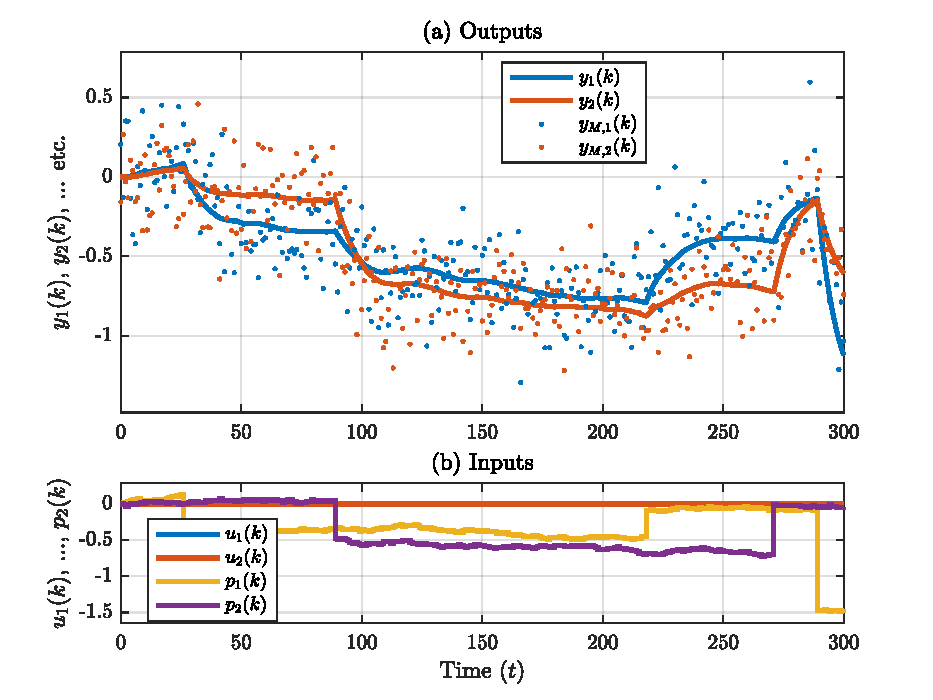
\includegraphics[width=13cm]{images/rod_obs_sim2_all_seed_ioplot.pdf}
	\caption{Simulation of linear MIMO system with two \gls{RODD}s}
	\label{fig:rod-obs-sim-2-ioplot}
\end{figure}

\begin{figure}[htp]
	\centering
	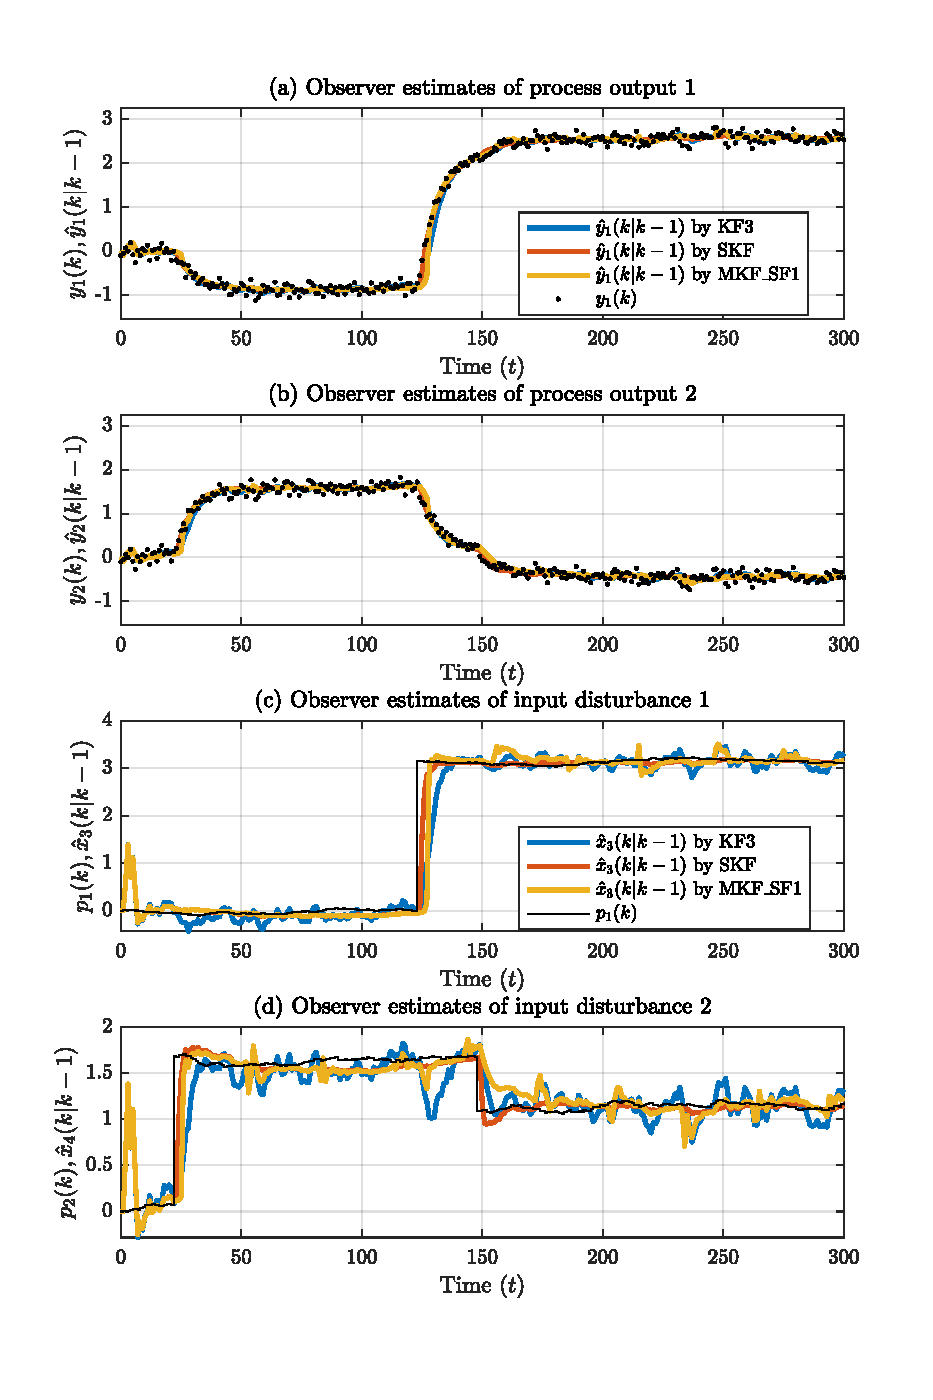
\includegraphics[width=13cm]{images/rod_obs_sim2_all_seed_y_est1_SF1.pdf}
	\caption{Estimates by sequence fusion observer –  $2\times2$ system}
	\label{fig:rod-obs-sim2-yest-1-SF}
\end{figure}

\begin{figure}[htp]
	\centering
	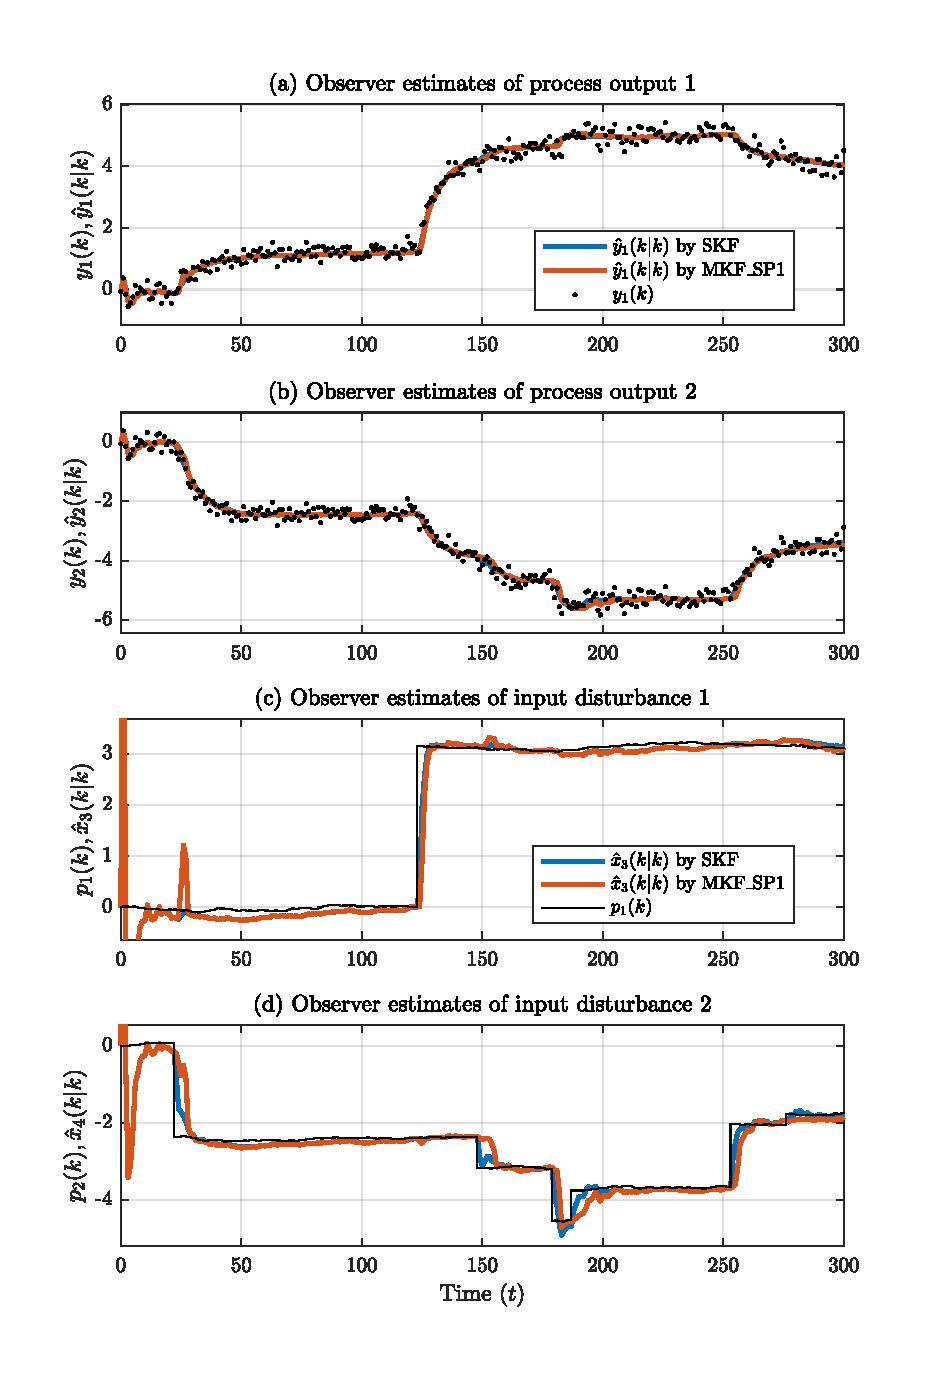
\includegraphics[width=13cm]{images/rod_obs_sim2_all_seed_y_est1_SP1.pdf}
	\caption{Estimates by sequence pruning observer –  $2\times2$ system}
	\label{fig:rod-obs-sim2-yest-1-SP}
\end{figure}

%\begin{figure}[htp]
%	\centering
%	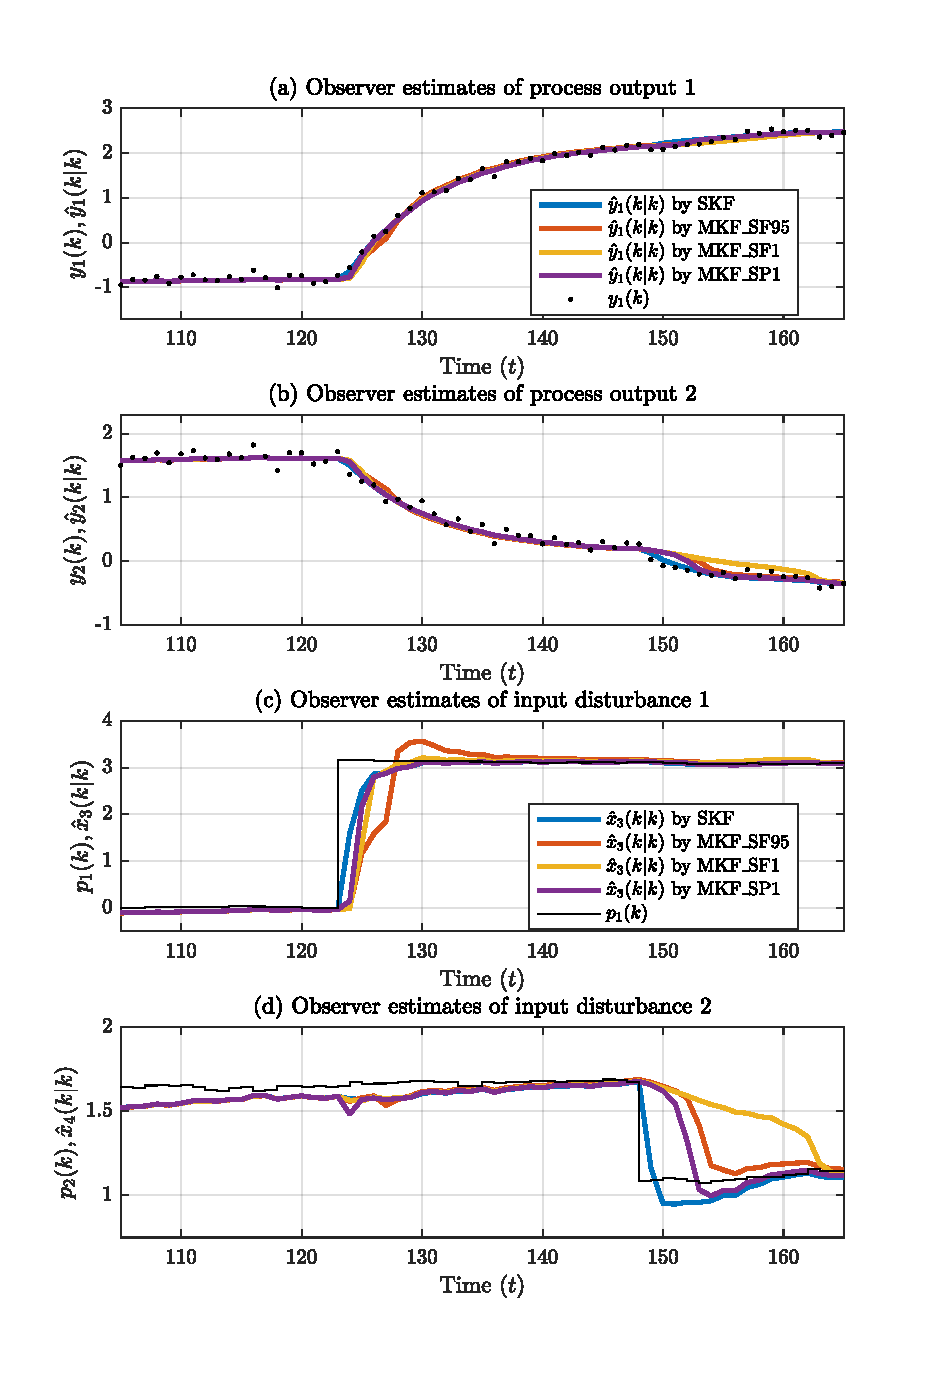
\includegraphics[width=13cm]{images/rod_obs_sim2_all_seed_y_est2_MKF.pdf}
%	\caption{Comparison of multi-model observer estimates –  $2\times2$ system}
%	\label{fig:rod-obs-sim2-yest-2-MKF}
%\end{figure}
\begin{figure}[htp]
	\centering
	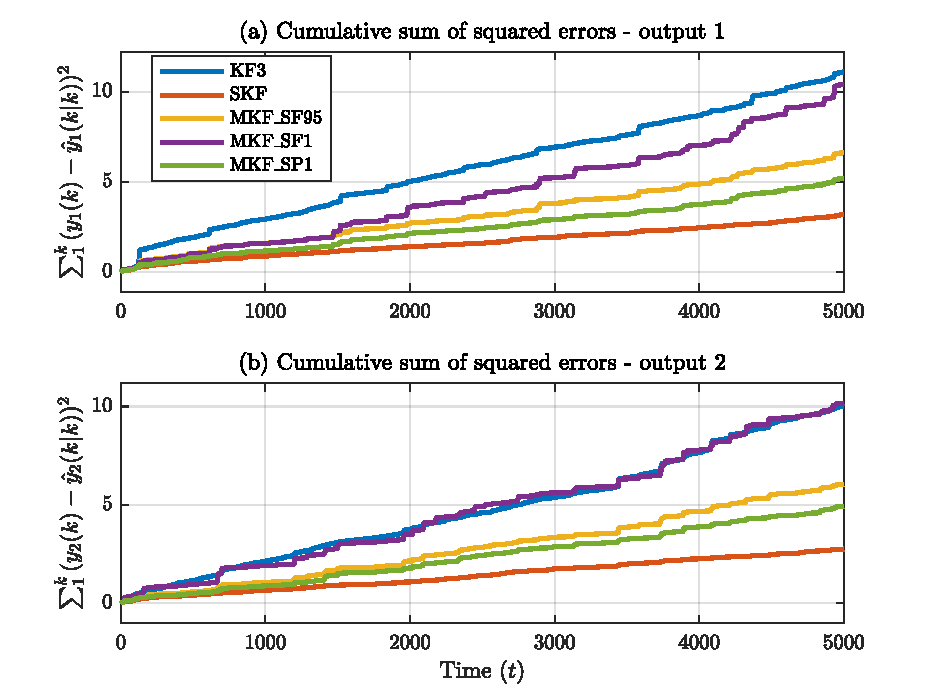
\includegraphics[width=13cm]{images/rod_obs_sim2_cum_err.pdf}
	\caption{Cumulative sum of squared errors of output estimates –  $2\times2$ system}
	\label{fig:sim-sys-sim2-MKF-cumerr}
\end{figure}

% Replaced with above single plot to save space
%\begin{figure}[htp]
%	\centering
%	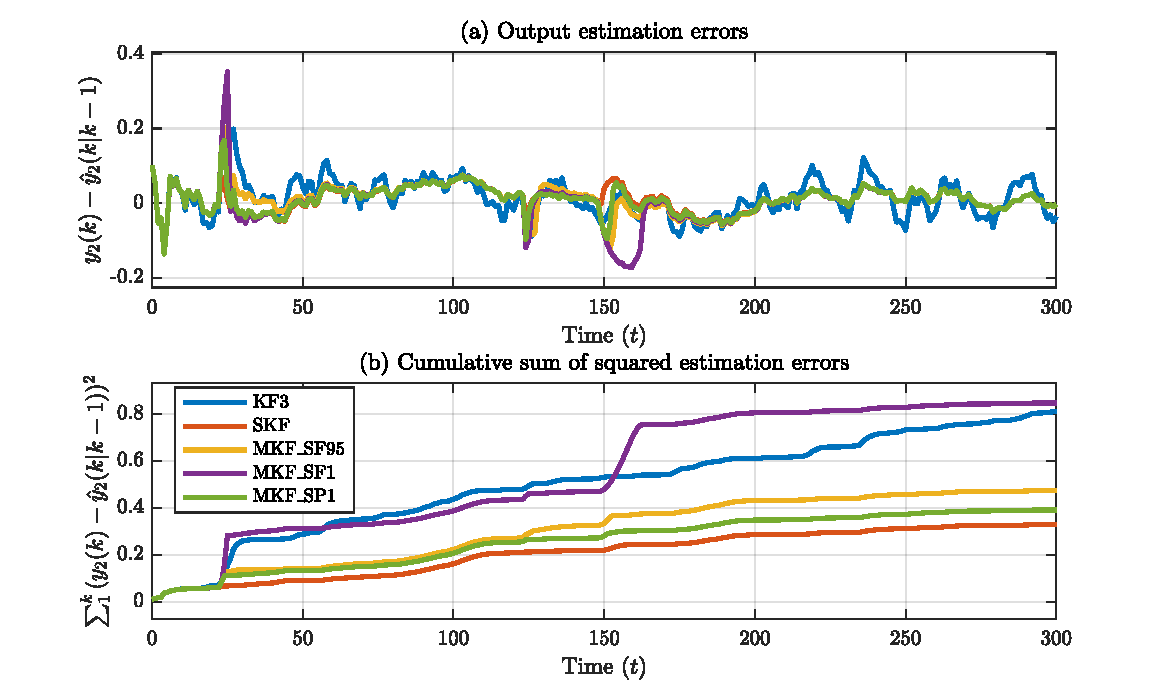
\includegraphics[width=13cm]{images/rod_obs_sim2_cum_err2.pdf}
%	\caption{Cumulative errors of multi-model observer output estimates –  $2\times2$ system}
%	\label{fig:sim-sys-sim2-MKF-cumerr2}
%\end{figure}

%\begin{figure}[htp]
%	\centering
%	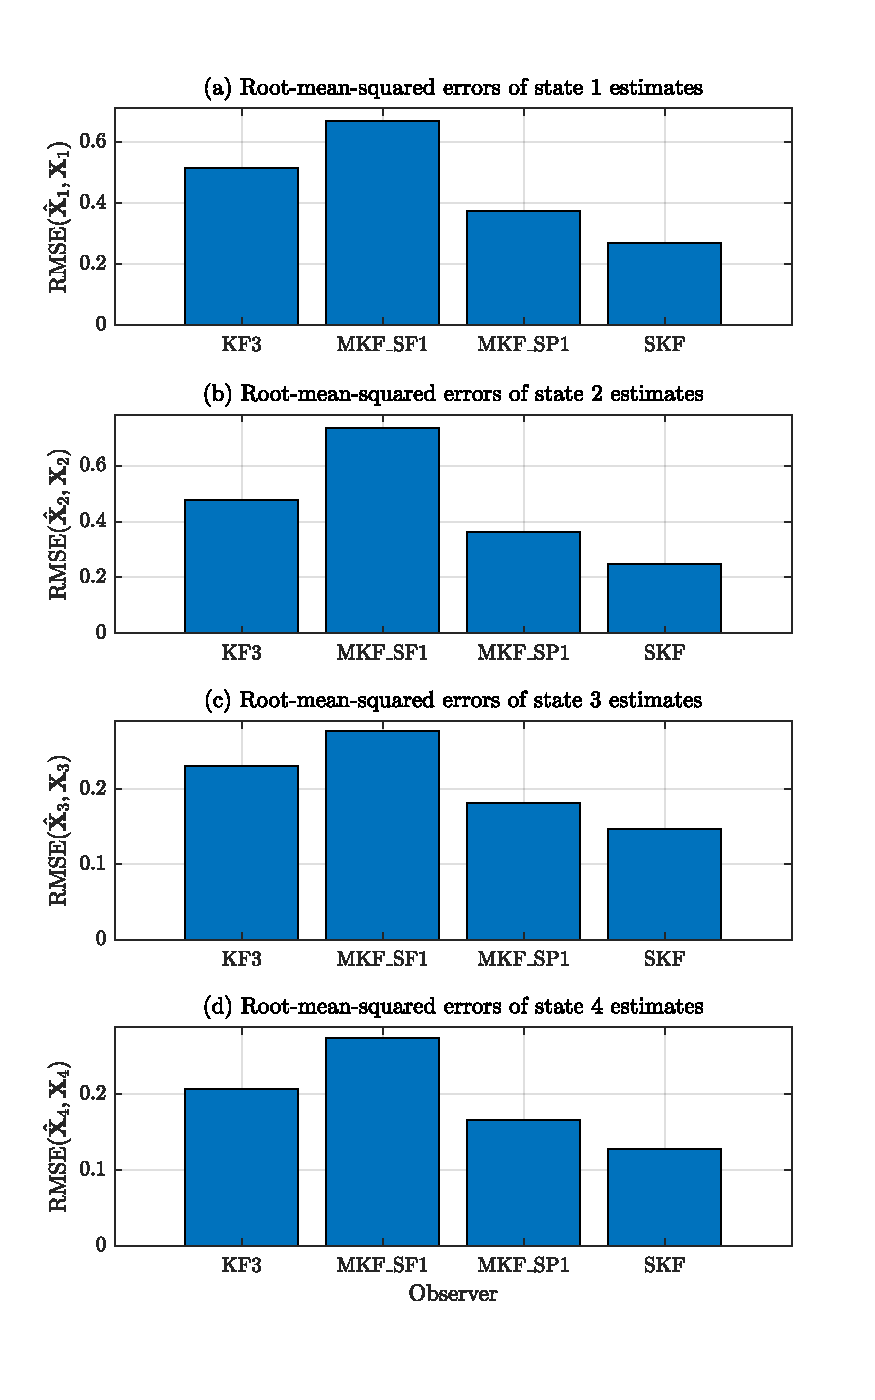
\includegraphics[width=11cm]{images/rod_obs_sim2_all_seed_x_err_bar.pdf}
%	\caption{Root-mean-squared errors of state estimates – $2\times2$ system}
%	\label{fig:rod-obs-sim2-xest-RMSE-bar}
%\end{figure}

\begin{figure}[htp]
	\centering
	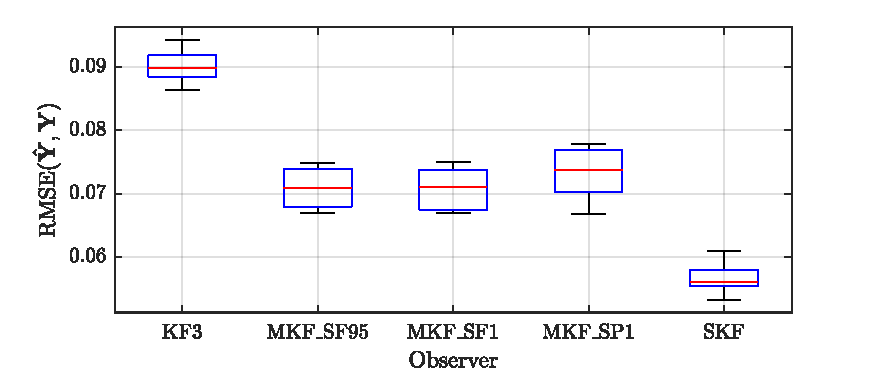
\includegraphics[width=11cm]{images/rod_obs_sim2_all_seed_y_err_box.pdf}
	\caption{Root-mean-squared errors of output estimates – $2\times2$ system}
	\label{fig:rod-obs-sim2-yest-all-seed-RMSE-box}
\end{figure}

\begin{table}[hb]
	\begin{center}
		\caption{Multi-model observer parameter search results – MKF--SF95.} \label{tb:obs-sim2-popt-SF95}
		% See: https://texblog.org/2019/06/03/control-the-width-of-table-columns-tabular-in-latex/
		\begin{tabular}{p{0.05\textwidth}>{\centering\arraybackslash}p{0.07\textwidth}>{\centering\arraybackslash}p{0.07\textwidth}>{\centering\arraybackslash}p{0.07\textwidth}>{\centering\arraybackslash}p{0.07\textwidth}>{\centering\arraybackslash}p{0.24\textwidth}}
			\gls{nf} & \gls{m}  & \gls{d}  & \gls{nh} & $\beta$ & $\operatorname{RMSE}(\hat{Y}(N),Y(N))$  \\
			\hline
			% Results with seed = 0, sigma_M = [0.2 0.2], d_min = 1
%			10 &   2 &   1 & 331 & 0.9990 & 0.0644 \\
%			6 &   2 &   2 &  22 & 0.8863 & 0.0670 \\
%			6 &   3 &   2 &  42 & 0.8864 & 0.0670 \\
%			5 &   3 &   1 & 452 & 1.0000 & 0.0680 \\
%			5 &   2 &   1 & 116 & 0.9999 & 0.0681 \\
%			6 &   1 &   2 &   7 & 0.8835 & 0.0683 \\
%			10 &   1 &   1 &  27 & 0.9841 & 0.0684 \\
%			5 &   1 &   1 &  17 & 0.9962 & 0.0688 \\
%			15 &   1 &   1 &  37 & 0.9653 & 0.0713 \\
%			3 &   3 &   1 & 138 & 1.0000 & 0.0739 \\
			% See script rod_obs_sim2_MKF_SF95_popt_table.m
			% 30-Nov-2022 17:56:06 results with seed = 0, sigma_M = [0.2 0.2], d_min = 1
%			20 &   2 &   2 & 211 & 0.9930 & 0.0640 \\
%			15 &   3 &   3 & 452 & 0.9999 & 0.0644 \\
%			10 &   2 &   1 & 331 & 0.9990 & 0.0644 \\
%			30 &   2 &   3 & 331 & 0.9795 & 0.0644 \\
%			15 &   2 &   3 & 116 & 0.9973 & 0.0644 \\
%			10 &   2 &   2 &  56 & 0.9991 & 0.0646 \\
%			10 &   3 &   2 & 176 & 1.0000 & 0.0646 \\
%			25 &   3 &   5 & 176 & 0.9990 & 0.0648 \\
%			15 &   2 &   5 &  22 & 0.9979 & 0.0649 \\
%			9 &   2 &   3 &  58 & 0.9995 & 0.0649 \\
			% See script rod_obs_sim3_MKF_SF95_popt_table.m
			% 01-Dec-2022 15:04:33 results with seed = 0, sigma_M = [0.2 0.2], d_min = 1
			30 &   2 &   3 & 331 & 0.9795 & 0.0877 \\
			15 &   2 &   3 & 116 & 0.9973 & 0.0878 \\
			15 &   3 &   3 & 452 & 0.9999 & 0.0880 \\
			9 &   1 &   3 &  13 & 0.9904 & 0.0882 \\
			20 &   2 &   2 & 211 & 0.9930 & 0.0887 \\
			9 &   2 &   3 &  58 & 0.9995 & 0.0887 \\
			9 &   3 &   3 & 138 & 1.0000 & 0.0888 \\
			10 &   1 &   1 &  27 & 0.9841 & 0.0888 \\
			10 &   2 &   1 & 331 & 0.9990 & 0.0889 \\
			10 &   1 &   2 &  11 & 0.9859 & 0.0892 \\
			\hline
		\end{tabular}
	\end{center}
\end{table}

\begin{table}[hb]
	\begin{center}
		\caption{Multi-model observer parameter search results – MKF--SF98.} \label{tb:obs-sim2-popt-SF98}
		% See: https://texblog.org/2019/06/03/control-the-width-of-table-columns-tabular-in-latex/
		\begin{tabular}{p{0.05\textwidth}>{\centering\arraybackslash}p{0.07\textwidth}>{\centering\arraybackslash}p{0.07\textwidth}>{\centering\arraybackslash}p{0.07\textwidth}>{\centering\arraybackslash}p{0.07\textwidth}>{\centering\arraybackslash}p{0.24\textwidth}}
			\gls{nf} & \gls{m}  & \gls{d}  & \gls{nh} & $\beta$ & $\operatorname{RMSE}(\hat{Y}(N),Y(N))$  \\
			\hline
			% See script rod_obs_sim2_MKF_SF98_popt_table.m
			% 30-Nov-2022 18:04:56 results with seed = 0, sigma_M = [0.2 0.2], d_min = 1
%			10 &   2 &   1 & 331 & 0.9990 & 0.0644 \\
%			5 &   3 &   1 & 452 & 1.0000 & 0.0680 \\
%			5 &   2 &   1 & 116 & 0.9999 & 0.0681 \\
%			10 &   1 &   1 &  27 & 0.9841 & 0.0684 \\
%			5 &   1 &   1 &  17 & 0.9962 & 0.0688 \\
%			15 &   1 &   1 &  37 & 0.9653 & 0.0713 \\
%			3 &   3 &   1 & 138 & 1.0000 & 0.0739 \\
%			3 &   2 &   1 &  58 & 1.0000 & 0.0740 \\
%			3 &   1 &   1 &  13 & 0.9988 & 0.0743 \\
%			20 &   1 &   1 &  47 & 0.9411 & 0.0759 \\
%			% 29-Nov-2022 18:55:40 results with seed = 0, sigma_M = [0.2 0.2], d_min = 2
%			10 &   2 &   2 & 331 & 0.9930 & 0.0782 \\
%			5 &   3 &   2 & 452 & 1.0000 & 0.0791 \\
%			5 &   2 &   2 & 116 & 0.9991 & 0.0791 \\
%			5 &   1 &   2 &  17 & 0.9859 & 0.0832 \\
%			3 &   3 &   2 & 138 & 1.0000 & 0.0834 \\
%			3 &   2 &   2 &  58 & 0.9998 & 0.0834 \\
%			3 &   1 &   2 &  13 & 0.9956 & 0.0864 \\
%			10 &   2 &   3 & 331 & 0.9795 & 0.0878 \\
%			10 &   1 &   2 &  27 & 0.9444 & 0.0881 \\
%			5 &   3 &   3 & 452 & 0.9999 & 0.0882 \\
			% See script rod_obs_sim3_MKF_SF98_popt_table.m
			% 01-Dec-2022 15:08:41 results with seed = 0, sigma_M = [0.2 0.2], d_min = 1
			20 &   2 &   2 & 331 & 0.9930 & 0.0888 \\
			10 &   1 &   1 &  27 & 0.9841 & 0.0888 \\
			10 &   2 &   1 & 331 & 0.9990 & 0.0889 \\
			10 &   3 &   2 & 452 & 1.0000 & 0.0891 \\
			10 &   2 &   2 & 116 & 0.9991 & 0.0891 \\
			10 &   1 &   2 &  17 & 0.9859 & 0.0898 \\
			6 &   3 &   2 & 138 & 1.0000 & 0.0904 \\
			6 &   2 &   2 &  58 & 0.9998 & 0.0904 \\
			6 &   1 &   2 &  13 & 0.9956 & 0.0905 \\
			15 &   1 &   1 &  37 & 0.9653 & 0.0907 \\
			\hline
		\end{tabular}
	\end{center}
\end{table}

\begin{table}[hb]
	\begin{center}
		\caption{Multi-model observer parameter search results – MKF--SP.} \label{tb:obs-sim2-popt-SP}
		% See: https://texblog.org/2019/06/03/control-the-width-of-table-columns-tabular-in-latex/
		\begin{tabular}{p{0.05\textwidth}>{\centering\arraybackslash}p{0.07\textwidth}>{\centering\arraybackslash}p{0.24\textwidth}}
			\gls{nh} & \gls{nmin} & $\operatorname{RMSE}(\hat{Y}(N),Y(N))$  \\
			\hline
			% 29-Nov-2022 18:31:09 results with seed = 0, sigma_M = [0.2 0.2]
%			14 &   6 & 0.0705  \\
%			32 &  12 & 0.0720  \\
%			32 &   9 & 0.0723  \\
%			25 &   5 & 0.0723  \\
%			32 &   5 & 0.0724  \\
%			25 &   6 & 0.0724  \\
%			25 &   1 & 0.0724  \\
%			32 &   7 & 0.0724  \\
%			32 &   4 & 0.0724  \\
%			32 &   6 & 0.0724  \\
			% See script rod_obs_sim3_MKF_SP_popt_table.m
			% 01-Dec-2022 15:07:09 results with seed = 0, sigma_M = [0.2 0.2]
			32 &   4 & 0.0875  \\
			32 &   3 & 0.0875  \\
			32 &   5 & 0.0876  \\
			32 &   6 & 0.0877  \\
			25 &   4 & 0.0877  \\
			32 &   2 & 0.0877  \\
			32 &   7 & 0.0878  \\
			25 &   5 & 0.0879  \\
			25 &   3 & 0.0879  \\
			25 &   2 & 0.0880  \\
		\end{tabular}
	\end{center}
\end{table}

\begin{table}[hb]
	\begin{center}
		\caption{Observer parameters for $2\times2$ linear system.} \label{tb:obs-params-sim2}
		% See: https://texblog.org/2019/06/03/control-the-width-of-table-columns-tabular-in-latex/
		\begin{tabular}{p{0.16\textwidth}>{\centering\arraybackslash}p{0.11\textwidth}>{\centering\arraybackslash}p{0.11\textwidth}>{\centering\arraybackslash}p{0.11\textwidth}>{\centering\arraybackslash}p{0.16\textwidth}>{\centering\arraybackslash}p{0.16\textwidth}}
			& KF1 & KF2 & KF3 & MKF--SF1 & MKF--SP1 \\
			\hline
			Type & Kalman filter & Kalman filter & Kalman filter & Multi-model Kalman filter & Multi-model Kalman filter \\
			Sub-optimal algorithm & - & - & - & Sequence fusion & Sequence pruning \\
			\hline
			Parameters &  &  &  & &  \\
			$\mathbf{Q}$ & $\mathbf{Q}_0$ & $\mathbf{Q}_1$ & $\mathbf{Q}_{opt}$ & $\{\mathbf{Q}_0,\mathbf{Q}_1\}$ & $\{\mathbf{Q}_0,\mathbf{Q}_1\}$ \\
			$\mathbf{R}$ & $\left[\begin{smallmatrix}0.1^2 & 0 \\ 0 & 0.1^2\end{smallmatrix}\right]$
				& $\left[\begin{smallmatrix}0.1^2 & 0 \\ 0 & 0.1^2\end{smallmatrix}\right]$
				& $\left[\begin{smallmatrix}0.1^2 & 0 \\ 0 & 0.1^2\end{smallmatrix}\right]$
				& $\left[\begin{smallmatrix}0.1^2 & 0 \\ 0 & 0.1^2\end{smallmatrix}\right]$
				& $\left[\begin{smallmatrix}0.1^2 & 0 \\ 0 & 0.1^2\end{smallmatrix}\right]$ \\
			$\mathbf{P}(0)$ & $\mathbf{P}_0$ & $\mathbf{P}_0$ & $\mathbf{P}_0$ & $\mathbf{P}_0$ & $\mathbf{P}_0$ \\
			\gls{nh} & 1 & 1 & 1 & 56 & 19 \\
			\gls{nf} & - & - & - & 25 & - \\
			\gls{m} & - & - & - & 2 & - \\
			\gls{d} & - & - & - & 5 & - \\
			\gls{nmin} & - & - & - & - & 5 \\
			\gls{epsilon} & - & - & - & 0.005 & 0.005 \\
			\gls{sigmawp} & - & - & - & 0.01 & 0.01 \\
			\gls{b} & - & - & - & 100 & 100 \\
			\hline
		\end{tabular}
	\end{center}
\end{table}

From these results, it was concluded that the multi-model observer proposed by \cite{robertson_method_1998} was not a good state estimator for this SISO system with one \gls{RODD} step disturbance. The sequence pruning algorithm proposed by \cite{eriksson_classification_1996}, on the other hand, seems to be a very good state estimator, significantly better than a single, well tuned Kalman filter.

\begin{itemize}
	\item Summary table comparing performance metrics for all three observers (KF3, MKF-SF, MKF-SP) - metrics: MSE, MSE-transitions, MSE-steady-state, variance-steady-state, MSD-steady-state.
	\item Discussion: Compare and contrast -> sequence pruning approach (Eriksson and Isaksson) works better.
	\item Conclude on pros, cons of each algorithm and decision to use sequence pruning for grinding simulation experiments.
\end{itemize}

\section{Ore feed disturbance estimation} \label{section:sim-ore-SISO}

Outline notes:
\begin{outline}
	\1 Unlike previous simulations, this is a non-linear model.
	\1 Describe simulations with grinding simulation model with changing ore properties and changes (same as IFAC paper).
	\1 Describe various data sets generated and their intended use (estimation, validation, statistical performance evaluation).
	\1 Data set used for model identification in Figure: Input-output data – Figure \ref{fig:rod_obs_sim_1_ioplot_P2DcTd4}.
	\1 How process model was identified.
	\1 Augmented model with \gls{RODD} input step disturbance.
	\1 Use best observer from previous section (sequence pruning).
	\1 Table showing observer parameters.
	\1 Figure: comparison of observer estimates – Figure \ref{fig:rod_obs_sim_1_est_P2DcTd4}.
	\1 Figure: Observer responses to disturbances – Figure \ref{fig:sim_resp_plot}.
	\1 Describe overall performance comparison using metrics in Table \ref{tb:results}.
	\1 Discuss pro's and con's of MKF observer (steady-state errors vs error in transitions, etc.)
	\1 Discuss applications and potential benefits (e.g. process control, RTO).
	\1 Describe sensitivity analysis simulations.
	\1 Describe sensitivity results:
	\2 (1) to model error, compare Kalman filter and MKF. Figures \ref{fig:rod_obs_sim_sens_model_KF2_MSE_y_est} and \ref{fig:rod_obs_sim_sens_model_MKF_MSE_y_est}.
	\2 (2) MKF sensitivity to \gls{RODD} model parameters. Figure  \ref{fig:rod_obs_sim_sens_rod_MKF_MSE_y_est}
\end{outline}

\begin{figure}[htp]
	\centering
	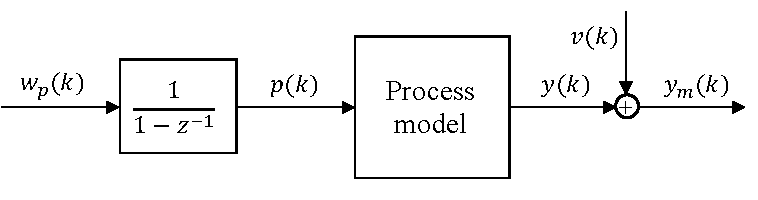
\includegraphics[width=10cm]{images/obs-model-diag.pdf}
	\caption{Observer model structure}
	\label{fig:obs_model}
\end{figure}

\begin{figure}[htp]
	\centering
	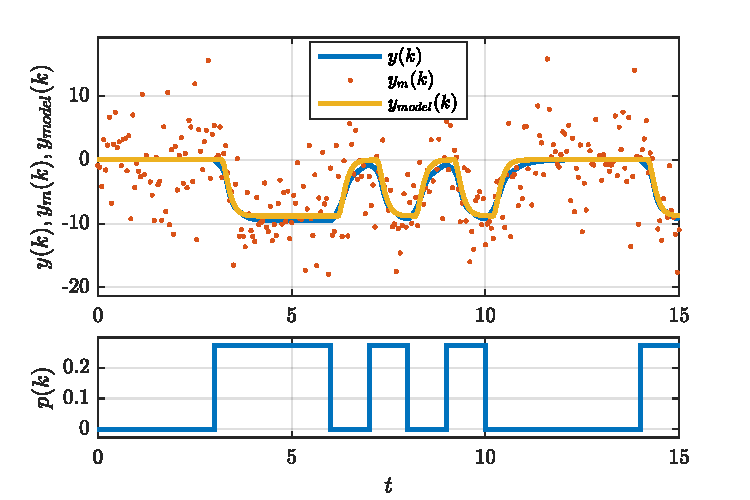
\includegraphics[width=12cm]{images/rod_obs_sim_1_ioplot_P2DcTd4.pdf}
	\caption{Grinding process simulation data and model estimates}
	\label{fig:rod_obs_sim_1_ioplot_P2DcTd4}
\end{figure}

\begin{figure}[htp]
	\centering
	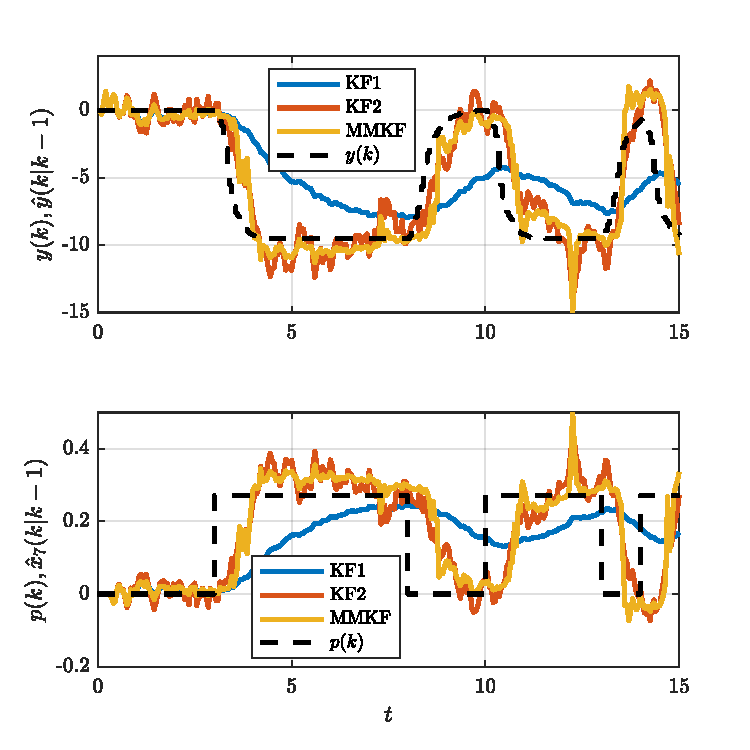
\includegraphics[width=12cm]{images/rod_obs_sim_1_est_P2DcTd4.pdf}
	\caption{Observer estimates}
	\label{fig:rod_obs_sim_1_est_P2DcTd4}
\end{figure}

\begin{figure}[htp]
	\centering
	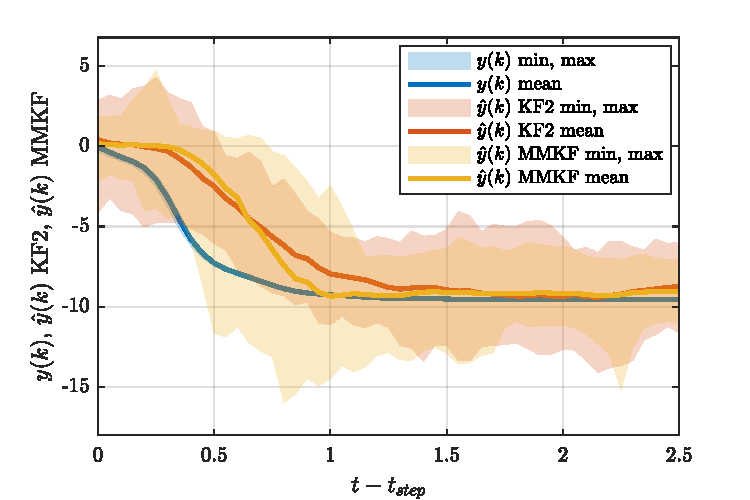
\includegraphics[width=12cm]{images/sim_resp_plot1_P2DcTd4.pdf}
	\caption{Average observer responses to step disturbances}
	\label{fig:sim_resp_plot}
\end{figure}

\begin{table}[hb]
	\begin{center}
		\caption{Observer performance evaluation metrics.} \label{tb:results}
		% See: https://texblog.org/2019/06/03/control-the-width-of-table-columns-tabular-in-latex/
		\begin{tabular}{p{0.34\textwidth}>{\centering\arraybackslash}p{0.09\textwidth}>{\centering\arraybackslash}p{0.09\textwidth}>{\centering\arraybackslash}p{0.09\textwidth}>{\centering\arraybackslash}p{0.11\textwidth}>{\centering\arraybackslash}p{0.09\textwidth}}
			Metric & KF1 & KF2 & KF3 & MKF-SP & SKF \\
			\hline
			MSE($\hat{y}(k),y(k)$) overall          & 11.0 & 15.9 & 3.7 & 3.5 & 2.1 \\ 
			MSE($\hat{y}(k),y(k)$) transient       & 21.1 & 16.1 & 7.7 & 11.2 & 5.1 \\ 
			MSE($\hat{y}(k),y(k)$) steady-state & 7.9 & 15.9 & 2.5 & 1.1 & 1.1 \\ 
			Var($\hat{y}(k)$) steady-state          & 1.8 & 15.3 & 1.9 & 0.5 & 0.2 \\ 
			MSD($\hat{y}(k),y(k)$) steady-state       & 0.0 & 16.2 & 0.5 & 0.2 & 0.0 \\ 
			% Results for P2DcTd4
			%  Gc = -32.4 * exp(-0.2 * s) / (1 + 0.106*s)^2;
			%                                 KF1       KF3       AFMM        SKF  
			%  MSE                         11.118    3.7395     3.6991     2.0615
			%  MSE in transitions          20.687    7.7201      12.18     5.0674
			%  MSE in steady-state         8.1885     2.521     1.1028     1.1414
			%  Variance in steady-state    1.7723    1.9026    0.39281    0.23769
			%
			% Results for P2Dcd1_T
			%  Gc = -35.94 * exp(-0.05 * s) / ((1 + 0.235*s) * (1 + 0.161*s));
			%                                 KF1       KF3       AFMM        SKF  
			%  MSE                         10.707    3.7702     3.7283     1.9652
			%  MSE in transitions          21.052    7.7605     12.397     4.8145
			%  MSE in steady-state         7.5404    2.5486     1.0745      1.093
			%  Variance in steady-state    1.8111    1.9259    0.39282    0.24514
			
			% Updated results for P2DcTd4 with n_filt = 20, n_min = 18 after fixing
			% initialization between MC simulation runs.
			%  MSE                          11.01    3.6869     3.4952     1.8191
			%  MSE in transitions          21.137    7.7201     11.208     5.0722
			%  MSE in steady-state         7.9091    2.4523     1.1342     0.8232
			%  Variance in steady-state    1.8008    1.9026    0.47604    0.23759
			
			\hline
		\end{tabular}
	\end{center}
\end{table}

\begin{figure}[htp]
	\centering
	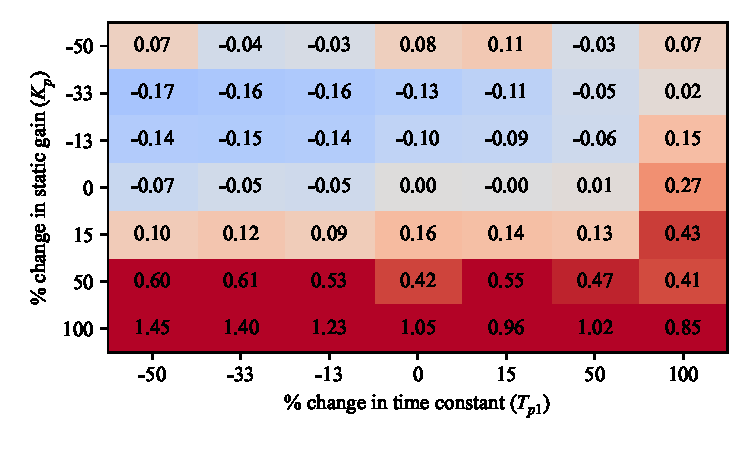
\includegraphics[width=12cm]{images/rod_obs_sim_sens_model_KF2_MSE_y_est.pdf}
	\caption{Sensitivity of KF2 estimates to changes in model parameters}
	\label{fig:rod_obs_sim_sens_model_KF2_MSE_y_est}
\end{figure}

\begin{figure}[htp]
	\centering
	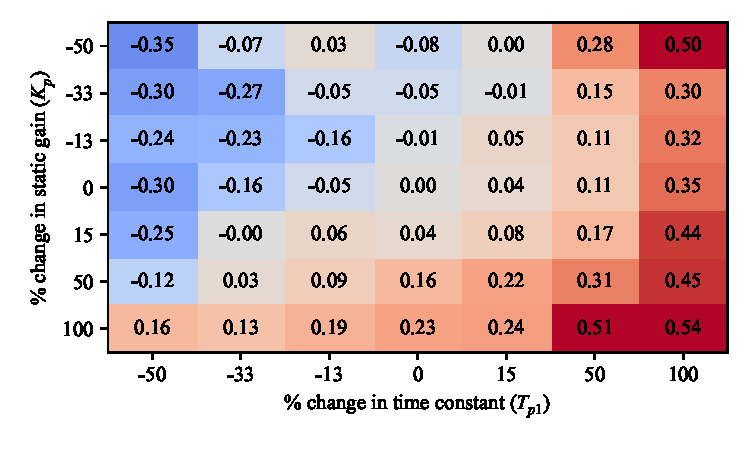
\includegraphics[width=12cm]{images/rod_obs_sim_sens_model_MKF_MSE_y_est.pdf}
	\caption{Sensitivity of \gls{MKF} observer estimates to changes in model parameters}
	\label{fig:rod_obs_sim_sens_model_MKF_MSE_y_est}
\end{figure}

\begin{figure}[htp]
	\centering
	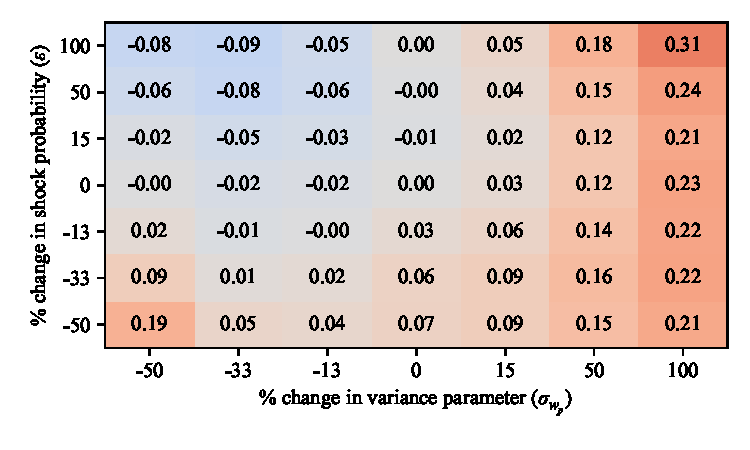
\includegraphics[width=12cm]{images/rod_obs_sim_sens_rod_MKF_MSE_y_est.pdf}
	\caption{Sensitivity of \gls{MKF} observer estimates to changes in \gls{RODD} parameters}
	\label{fig:rod_obs_sim_sens_rod_MKF_MSE_y_est}
\end{figure}


\section{Grinding circuit control simulation} \label{section:sim-ore-mimo-ctrl} 

Outline notes:
\begin{itemize}
	\item Grinding simulation model in closed loop with \gls{MPC} controller.
	\item Diagram of feedback system – Figure \ref{fig:sim-mpc-diag}
	\item Table of results - Performance metrics — e.g. tracking error.
	\item Robustness?  E.g. stability margins.
\end{itemize}

\begin{figure}[htp]
	\centering
	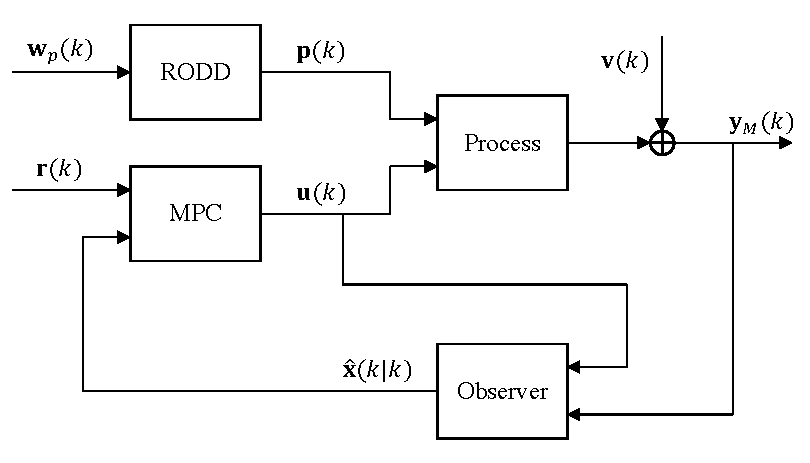
\includegraphics[width=11cm]{images/sim-mpc-diag.pdf}
	\caption{Functional diagram of the simulated feedback control system}
	\label{fig:sim-mpc-diag}
\end{figure}

\begin{figure}[htp]
	\centering
	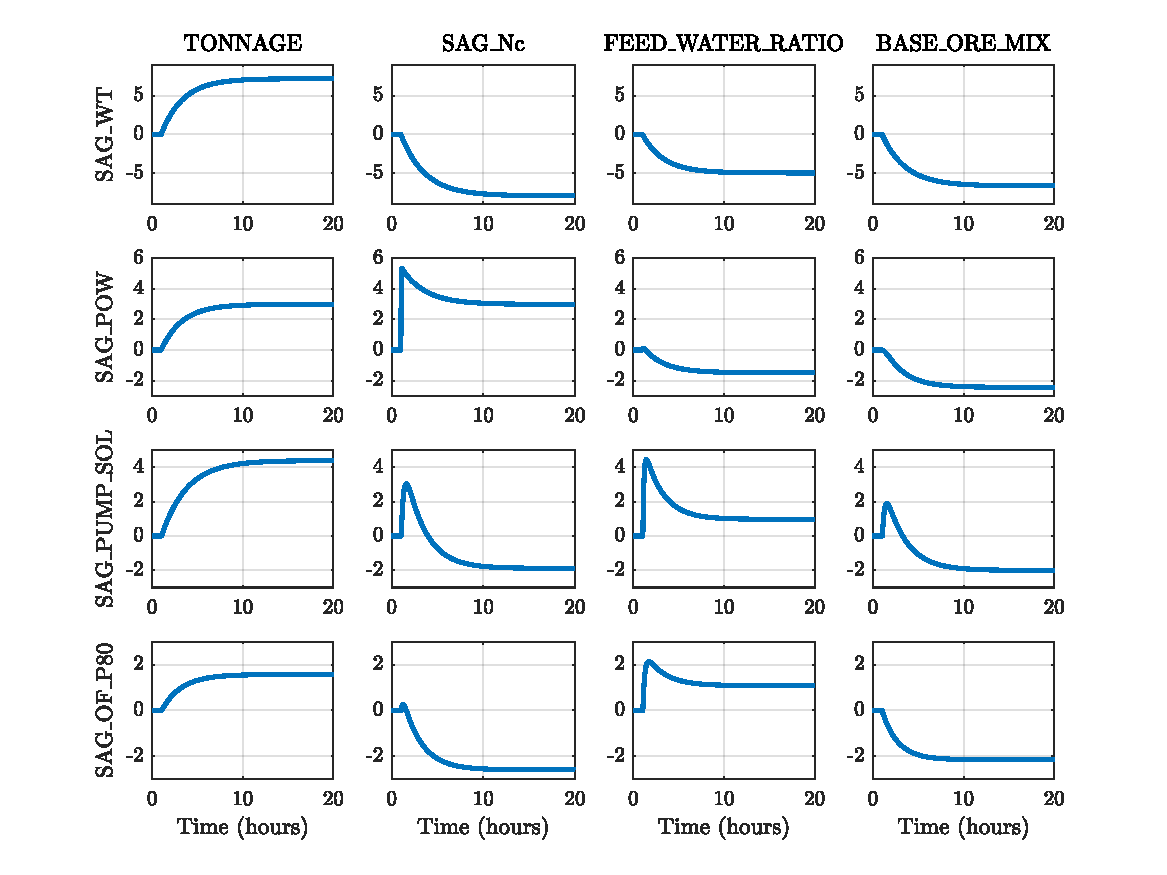
\includegraphics[width=15.5cm]{images/mpc4x4_stepresp_matrix.pdf}
	\caption{Step responses of identified input-output model}
	\label{fig:mpc4x4-stepresp-matrix}
\end{figure}

